\documentclass[11pt,a4paper,oneside]{report}

% -----------------------------------------------------------------------------
% Edit only these four fields for submission.
% -----------------------------------------------------------------------------
\newcommand{\ReportAuthor}{Student Name}
\newcommand{\ReportProgramme}{M.Sc. Physics}
\newcommand{\ReportInstitution}{Institution Name}
\newcommand{\ReportSupervisor}{Supervisor Name}

\usepackage[a4paper,top=22mm,bottom=22mm,left=25mm,right=20mm]{geometry}
\usepackage[T1]{fontenc}
\usepackage[utf8]{inputenc}
\usepackage{lmodern}
\usepackage{microtype}
\usepackage{amsmath,amssymb,bm}
\usepackage{booktabs,tabularx,array,multirow}
\usepackage{arydshln}
\usepackage{graphicx}
\usepackage{float}
\usepackage{caption}
\usepackage{subcaption}
\usepackage{siunitx}
\usepackage{xcolor}
\usepackage{enumitem}
\usepackage{fancyhdr}
\usepackage{titlesec}
\usepackage[hidelinks]{hyperref}
\usepackage[nameinlink,noabbrev]{cleveref}

\graphicspath{{figures/}}
\sisetup{detect-all,group-separator={,},group-minimum-digits=4,group-digits=integer}
\setlength{\parindent}{1.25em}
\setlength{\parskip}{0.2em}
\setlist{nosep,leftmargin=1.7em}
\captionsetup{font=small,labelfont=bf}
\setlength{\textfloatsep}{9pt plus 2pt minus 2pt}
\setlength{\floatsep}{8pt plus 2pt minus 2pt}
\setlength{\intextsep}{8pt plus 2pt minus 2pt}
\renewcommand{\topfraction}{0.92}
\renewcommand{\bottomfraction}{0.85}
\renewcommand{\textfraction}{0.08}
\renewcommand{\floatpagefraction}{0.82}
\setlength{\arrayrulewidth}{0.5pt}
\renewcommand{\arraystretch}{1.10}
\titleformat{\chapter}[display]
  {\normalfont\bfseries\Large}{\chaptertitlename\ \thechapter}{5pt}{\LARGE}
\titlespacing*{\chapter}{0pt}{-18pt}{14pt}
% \pagestyle{fancy}
% \fancyhf{}
% % \fancyhead[L]{GPU-Accelerated Urban Flood Modelling}
% \fancyhead[R]{\nouppercase{\leftmark}}
\fancyfoot[C]{\thepage}
\setlength{\headheight}{14pt}

\newcommand{\cupy}{CuPy/CUDA}
\newcommand{\jax}{JAX/XLA}
\newcommand{\sourcepkg}{\texttt{HF\_CUPY\_JAX\_COMPLETED\_PROJECT}}
\newcommand{\important}[1]{\textbf{#1}}
\newcommand{\projectsource}{\textit{Source: completed-project evidence package.}}
\newcommand{\anugasource}{\textit{Source: ANUGA controlled-case evidence.}}

\begin{document}
\pagenumbering{arabic}
\hypersetup{pageanchor=false}

% =============================================================================
% FRONT MATTER
% =============================================================================
\begin{titlepage}
  \thispagestyle{empty}
  \centering
  \vspace*{5mm}

  {\fontsize{24}{29}\selectfont\bfseries GPU-Accelerated Physics-Based\par}
  \vspace{1mm}
  {\fontsize{24}{29}\selectfont\bfseries Urban Flood Modelling\par}
  \vspace{5mm}
  {\large Using CuPy/CUDA and JAX/XLA\par}

  \vspace{17mm}
  {\large A Project Report submitted by\par}
  \vspace{6mm}
  {\large\bfseries Sanjeev Kumawat\par}
  \vspace{1mm}
  {\large M.Sc. Student, Indian Institute of Technology Hyderabad\par}

  \vspace{17mm}
  {\large in partial fulfilment of the requirements for the\par}
  \vspace{1mm}
  {\large INSPIRE Summer Project\par}

  \vspace{17mm}
  {\large Under the Guidance of\par}
  \vspace{6mm}
  {\large\bfseries Prof. Udit Bhatia\par}
  \vspace{1mm}
  {\large Associate Professor, Indian Institute of Gandhinagar\par}

  \vspace{16mm}
  \begin{minipage}[c]{0.28\textwidth}
    \centering
    
\includegraphics[height=29mm]{iitgn_logo.png}
  \end{minipage}
  \hspace{5mm}
  \begin{minipage}[c]{0.52\textwidth}
    \centering
    
\includegraphics[width=\linewidth]{iith_logo.png}
  \end{minipage}

  \vfill
  {\large August 2026\par}
  \vspace*{10mm}
\end{titlepage}
\hypersetup{pageanchor=true}
\setcounter{page}{2}

\chapter*{Declaration}
\addcontentsline{toc}{chapter}{Declaration}
\thispagestyle{empty}
I declare that this report presents the computational work and evidence contained in the
project archive identified in the reproducibility statement. Sources of theory and software
are acknowledged in the references. Numerical verification is distinguished throughout
from validation against observations; no unavailable measurements, simulations, or AI
results have been invented.

\vspace{12mm}
\begin{flushright}
\textbf{Sanjeev Kumawat}\\[1mm]
M.Sc. student\\
Department of Physics\\
Indian Institute of Technology Hyderabad
\end{flushright}

\vspace{18mm}
\noindent Date: 4 August 2026\\
Place: Gandhinagar
\clearpage

\chapter*{Acknowledgement}
\addcontentsline{toc}{chapter}{Acknowledgement}
\thispagestyle{empty}
I acknowledge the guidance of Prof. Udit Bhatia, the provision of the production domain and
forcing data, and the use of the external GPU system on which the reported production runs
were executed. The author remains responsible for the analysis and interpretation.

\vspace{12mm}
\begin{flushright}
\textbf{Sanjeev Kumawat}
\end{flushright}
\clearpage

\chapter*{Abstract}
\addcontentsline{toc}{chapter}{Abstract}
This project investigates whether one physics-based urban flood model can be implemented
consistently through two GPU programming systems: an explicit CuPy/CUDA implementation and
a compiled JAX/XLA implementation. Both backends solve the two-dimensional shallow-water
equations on the same unstructured triangular mesh and use the same terrain, spatially varying
Manning resistance, hydrostatic-reconstruction HLL flux, wetting and drying rules, Horton
infiltration, rainfall, recharge, drainage, surcharge, outfall, boundary and external-inflow
data. The production experiment covers 297.966 km$^2$ of active area with 981,880 triangles,
1,490,015 surface edges, 118,768 drainage nodes and 139,798 drainage links. A 160.09 mm,
24-hour rainfall event was simulated in single precision on one NVIDIA RTX PRO 4000 Blackwell
GPU without CPU fallback.

Cross-backend verification passed all eight approved numerical gates. The maximum hourly
depth root-mean-square error was 0.000979348 m, the minimum hourly flood-extent critical
success index was 0.998031, and maximum final depths differed by $7.63\times10^{-6}$ m.
Independent repeat runs showed RMSE values of 0.000416766 m for CuPy and 0.000406100 m
for JAX. The runs were therefore numerically repeatable within the registered criteria but
were not byte-for-byte identical. In a secondary 60-minute benchmark with three warm-up runs
and ten measurements per backend, median solver runtimes were 17.267 s for CuPy and 18.213 s
for JAX; JAX was 5.476\% slower for this workload. This result is not substituted for the
unfinished repeated 24-hour official benchmark. ANUGA was used only on small compatible
controlled cases as an independent numerical reference. No observational flood data were
available, and only one production event was available; consequently, physical validation,
production AI training and operational forecasting claims are outside the evidence. The
contribution is a tested, reproducible GPU numerical model and a scientifically qualified
comparison of its two accelerator implementations.

\medskip
\noindent\textbf{Code availability:} The implementation, experiment configurations,
verification evidence and report sources are available at
\url{https://github.com/arsanjeevk/gpu-urban-flood-cupy-jax}.

\noindent\textbf{Keywords:} shallow-water equations; urban flooding; GPU computing;
CuPy; CUDA; JAX; XLA; finite volume method; numerical verification; drainage coupling.
\clearpage

\tableofcontents
\clearpage
\chapter*{Lists of Figures and Tables}
\addcontentsline{toc}{chapter}{Lists of Figures and Tables}
\section*{Figures}
\makeatletter\@starttoc{lof}\makeatother
\vspace{5mm}
\section*{Tables}
\makeatletter\@starttoc{lot}\makeatother
\clearpage

\chapter*{Nomenclature}
\addcontentsline{toc}{chapter}{Nomenclature}
\begin{tabularx}{\textwidth}{|>{$}l<{$}|X|}
\hline
\multicolumn{1}{|l|}{\textbf{Symbol}} & \textbf{Meaning} \\
\hline\hline
h & Surface-water depth (m) \\ \hdashline[0.4pt/1.2pt]
u,v & Depth-averaged velocities in the projected $x$ and $y$ directions (m s$^{-1}$) \\ \hdashline[0.4pt/1.2pt]
hu,hv & Conserved depth-integrated momentum components (m$^2$ s$^{-1}$) \\ \hdashline[0.4pt/1.2pt]
z & Bed elevation (m, vertical datum undocumented) \\ \hdashline[0.4pt/1.2pt]
\bm U & Conserved surface state vector $[h,hu,hv]^{\mathsf T}$ \\ \hdashline[0.4pt/1.2pt]
\bm F,\bm G & Shallow-water flux vectors in the $x$ and $y$ directions \\ \hdashline[0.4pt/1.2pt]
\bm S & Combined physical and coupling source vector \\ \hdashline[0.4pt/1.2pt]
g & Gravitational acceleration, 9.80665 m s$^{-2}$ \\ \hdashline[0.4pt/1.2pt]
n & Manning resistance coefficient (s m$^{-1/3}$) \\ \hdashline[0.4pt/1.2pt]
r(t) & Piecewise-constant rainfall intensity (m s$^{-1}$ internally) \\ \hdashline[0.4pt/1.2pt]
f_0,f_c,k & Initial capacity, final capacity and decay coefficient in the Horton model \\ \hdashline[0.4pt/1.2pt]
A_i,L_e & Triangle area and edge length (m$^2$ and m) \\ \hdashline[0.4pt/1.2pt]
\Delta t & Adaptive explicit solver timestep (s) \\ \hdashline[0.4pt/1.2pt]
C_{\mathrm{CFL}} & Courant--Friedrichs--Lewy coefficient \\ \hdashline[0.4pt/1.2pt]
\operatorname{RMSE} & Root-mean-square error \\ \hdashline[0.4pt/1.2pt]
\operatorname{CSI} & Critical success index for thresholded flood extent \\
\hline
\end{tabularx}

\vspace{6mm}
\noindent\textbf{Backend abbreviations.} CUDA denotes NVIDIA's GPU execution platform;
CuPy denotes the NumPy-compatible CUDA array backend; JAX denotes the traced array-program
backend; and XLA denotes the compiler used to lower the staged JAX computation. ANUGA is an
external shallow-water reference and is not either production backend.
\clearpage
% =============================================================================
\chapter{Introduction}
% =============================================================================
\section{Motivation}

Urban flood simulation involves rapid overland flow, heterogeneous terrain, rainfall losses, drainage systems, and boundary exchanges. At city scale, the computational mesh can contain millions of interacting elements, while explicit time integration requires repeated local flux and source-term evaluations. Consequently, computational efficiency is a major challenge for high-resolution flood simulation.

GPU acceleration is a promising approach because many of these local operations can be executed concurrently. However, computational speed alone is insufficient for a scientifically meaningful implementation. An accelerated solver must preserve the governing equations, input data, numerical decisions, and physical behaviour of the reference formulation. Therefore, performance evaluation must be accompanied by systematic numerical-parity checks.

This study focuses specifically on two GPU acceleration approaches: \textbf{CuPy} and \textbf{JAX}. CuPy provides NumPy-compatible GPU operations and supports custom CUDA kernels, whereas JAX uses just-in-time compilation through XLA. Both approaches are evaluated on the same complete production dataset for the Gurugram application. The objective is to compare the execution performance of the two GPU implementations while maintaining numerical consistency with the reference flood-model formulation.

\section{Scientific and computational background}

The shallow-water equations are a depth-integrated approximation to free-surface flow. They
retain gravity-wave propagation and horizontal momentum transport while assuming that the
horizontal length scale is large relative to water depth. In conservation form they admit
discontinuities, moving wet--dry fronts and rapidly varying flow. A finite-volume method is
therefore appropriate because it updates cell-integrated quantities through edge fluxes and
can be constructed directly on an unstructured mesh \cite{leveque2002}. Triangular cells are
particularly useful in urban domains because they can follow irregular boundaries and local
geometric detail without imposing a rectangular grid over the entire region.

Numerical treatment of topography is central to flood modelling. A naive discretisation may
generate artificial motion even when the water surface should remain at rest. Hydrostatic
reconstruction modifies the left and right depths seen by an interface flux and adds matched
pressure corrections, providing a well-balanced treatment of bed steps while maintaining
non-negative reconstructed water depth \cite{audusse2004}. The HLL approximate Riemann
solver estimates the fastest left- and right-travelling signals and constructs one
conservative interface flux without explicitly resolving every characteristic wave
\cite{harten1983}. Wetting and drying rules then prevent division by vanishing depth.

Rainfall is not identical to effective surface input because part of it may infiltrate or
enter engineered drainage. The Horton relationship represents a capacity that decreases
from an initial value toward a final value as wet time accumulates \cite{horton1933}.
Surface resistance is represented through spatial Manning coefficients
\cite{chow1959}. In this study, these quantities participate in the production update
alongside recharge, inlet capture, pipe conveyance, surcharge, outfalls, and external
boundary inflow.

The computational structure exposes large groups of independent edge and cell operations,
but indexed accumulation and adaptive stepping complicate acceleration. CuPy permits direct
control of device arrays and custom CUDA kernels \cite{cupy}; JAX instead traces functional
array code and lets XLA compile the staged computation \cite{jax}. These approaches therefore
provide different computational mechanisms for executing the same underlying numerical
formulation, which motivates their evaluation under a common physical and computational
framework.

\section{Aim, objectives and research questions}

The aim of this study is to evaluate the numerical correctness, repeatability, and measured
execution performance of equivalent CuPy and JAX GPU implementations of a physics-based
urban flood model.

The study has four objectives:
\begin{enumerate}
    \item implement the production surface--drainage model using CuPy/CUDA and JAX/XLA;
    \item ensure that both implementations follow the same physical and numerical formulation;
    \item evaluate cross-backend numerical parity and within-backend repeatability; and
    \item compare their execution performance under a repeated and synchronized GPU protocol.
\end{enumerate}

These objectives lead to three research questions:

\begin{enumerate}
    \item Does the JAX implementation reproduce the CuPy reference within the predefined
    numerical acceptance criteria?
    
    \item Are repeated executions of each backend numerically stable within the predefined
    repeatability criteria, even when bitwise identity is not obtained?
    
    \item What execution-time difference is observed between the two implementations for an
    identical repeated GPU workload?
\end{enumerate}

\section{Scope and contribution}

The contribution of this study is numerical and computational rather than observational. The
production model includes complete terrain and roughness fields, shallow-water dynamics,
rainfall and Horton infiltration, recharge, dynamic drainage, surcharge, outfalls, external
hydrograph forcing, inactive-cell walls, and outflow-only exterior boundaries. The study
establishes software-test success, cross-backend numerical parity, within-backend
repeatability, and measured GPU performance for the CuPy and JAX implementations.

The study does not establish physical validation of the predicted inundation because compatible
observed depth, flood extent, discharge, or timing data were not available. The performance
results are also specific to the tested hardware, software environment, production dataset, and
benchmark protocol and should not be interpreted as a universal ranking of GPU frameworks.

\section{Report organisation}

Chapter 2 describes the production domain and forcing; Chapter 3 defines the physical and
numerical model; Chapter 4 explains the two GPU implementation paths; and Chapter 5
describes the verification and experimental methodology. Chapters 6 to 8 present the
production simulation, numerical parity and repeatability, and GPU performance results,
respectively. Chapter 9 provides the limited ANUGA numerical reference, followed by the
limitations and future work in Chapter 10 and the conclusions in Chapter 11.


% =============================================================================
\chapter{Production Data and Computational Domain}\label{chap:data}
% =============================================================================


\section{Domain construction}

The production surface is an unstructured triangular mesh in EPSG:32643. It contains 499,901
vertices and 981,880 triangles connected by 1,490,015 surface edges. Of these triangles, 817,573
are active and 164,307 are inactive; inactive cells act as closed walls. The active area is
297.965823~km$^2$. There are 34,390 exterior edges with code 4, treated as outflow-only except
where the historical external inflow is applied.

\begin{table}[htbp]
\centering
\caption{Production-domain inventory obtained from the packaged topology summary.}
\label{tab:domain_inventory}
\begin{tabular}{|l|r|l|r|}
\hline
\textbf{Quantity} & \textbf{Count} & \textbf{Quantity} & \textbf{Count} \\
\hline\hline
Mesh vertices & 499,901 & Surface edges & 1,490,015 \\ \hdashline[0.4pt/1.2pt]
All triangles & 981,880 & Active triangles & 817,573 \\ \hdashline[0.4pt/1.2pt]
Inactive triangles & 164,307 & Exterior code-4 edges & 34,390 \\ \hdashline[0.4pt/1.2pt]
Drainage nodes & 118,768 & Drainage links & 139,798 \\ \hdashline[0.4pt/1.2pt]
Mapped inlets & 61,317 & Enabled outfalls & 46 \\ \hdashline[0.4pt/1.2pt]
Recharge records & 447 & Hourly solver states & 25 \\
\hline
\end{tabular}
\end{table}



\begin{figure}[htbp]
\centering
\begin{subfigure}[t]{0.49\textwidth}
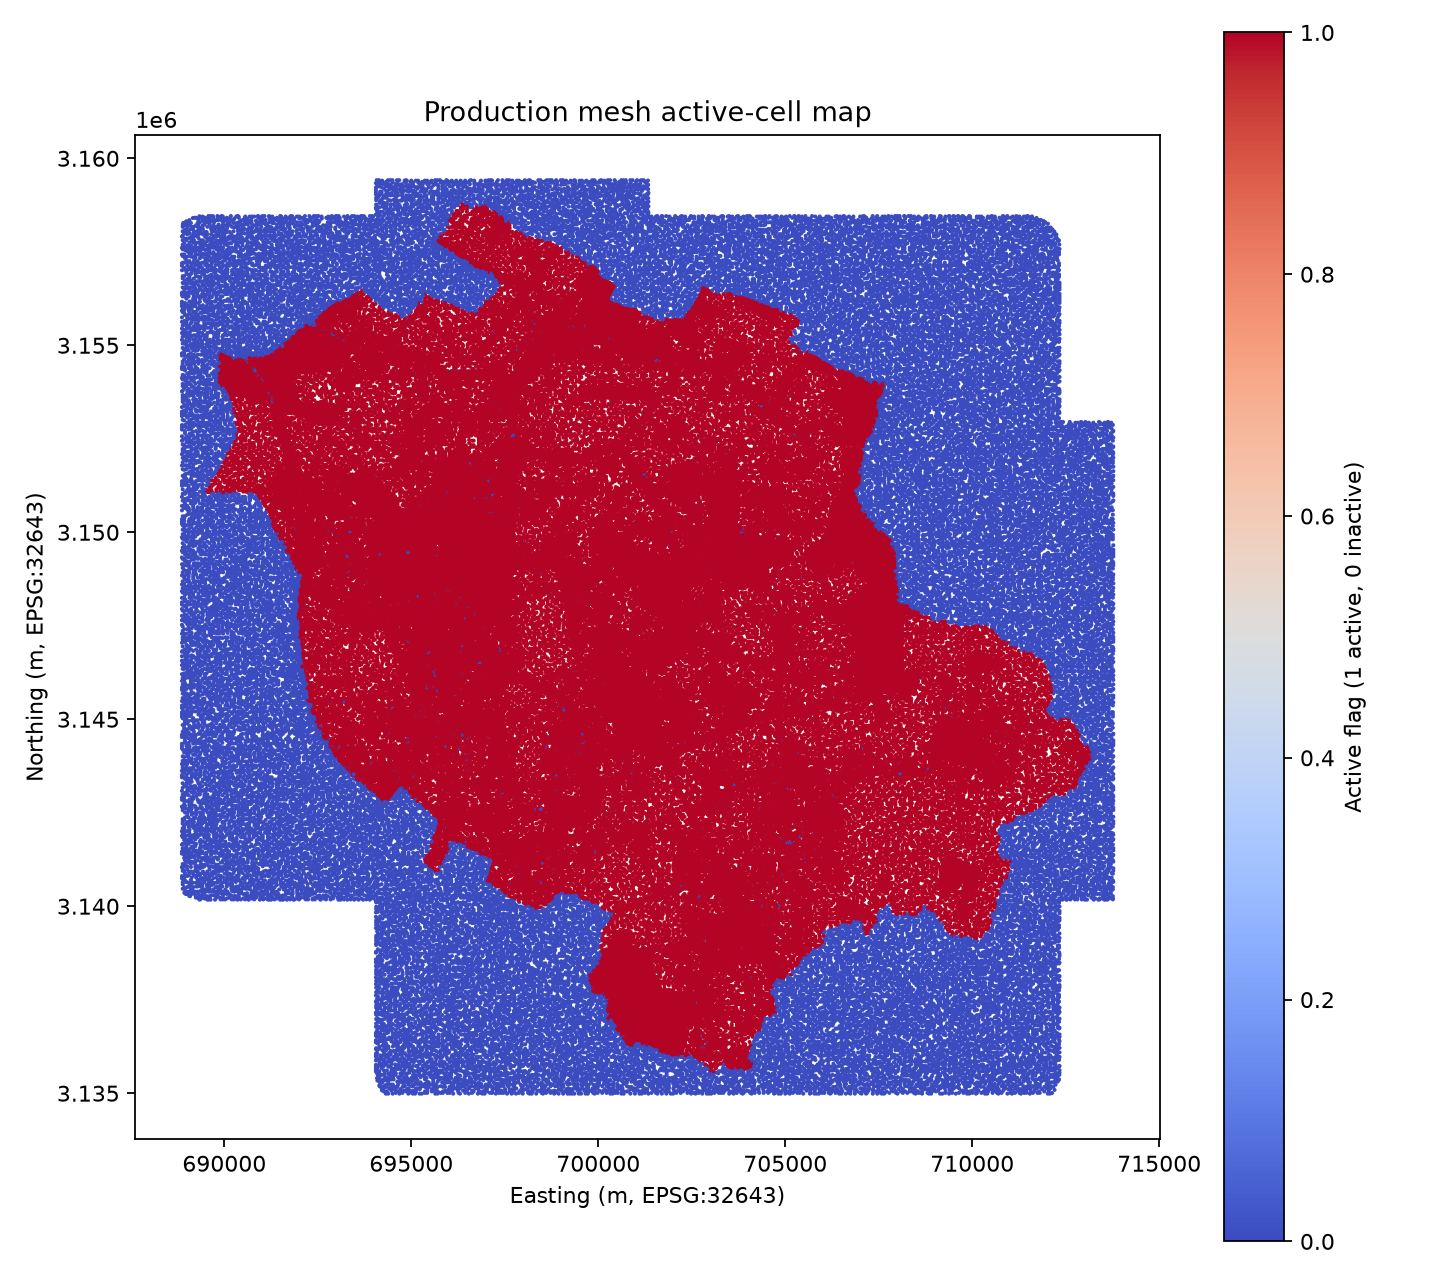
\includegraphics[width=\linewidth]{01_mesh_active_cells.png}
\caption{Active and inactive triangular cells.}
\end{subfigure}\hfill
\begin{subfigure}[t]{0.49\textwidth}
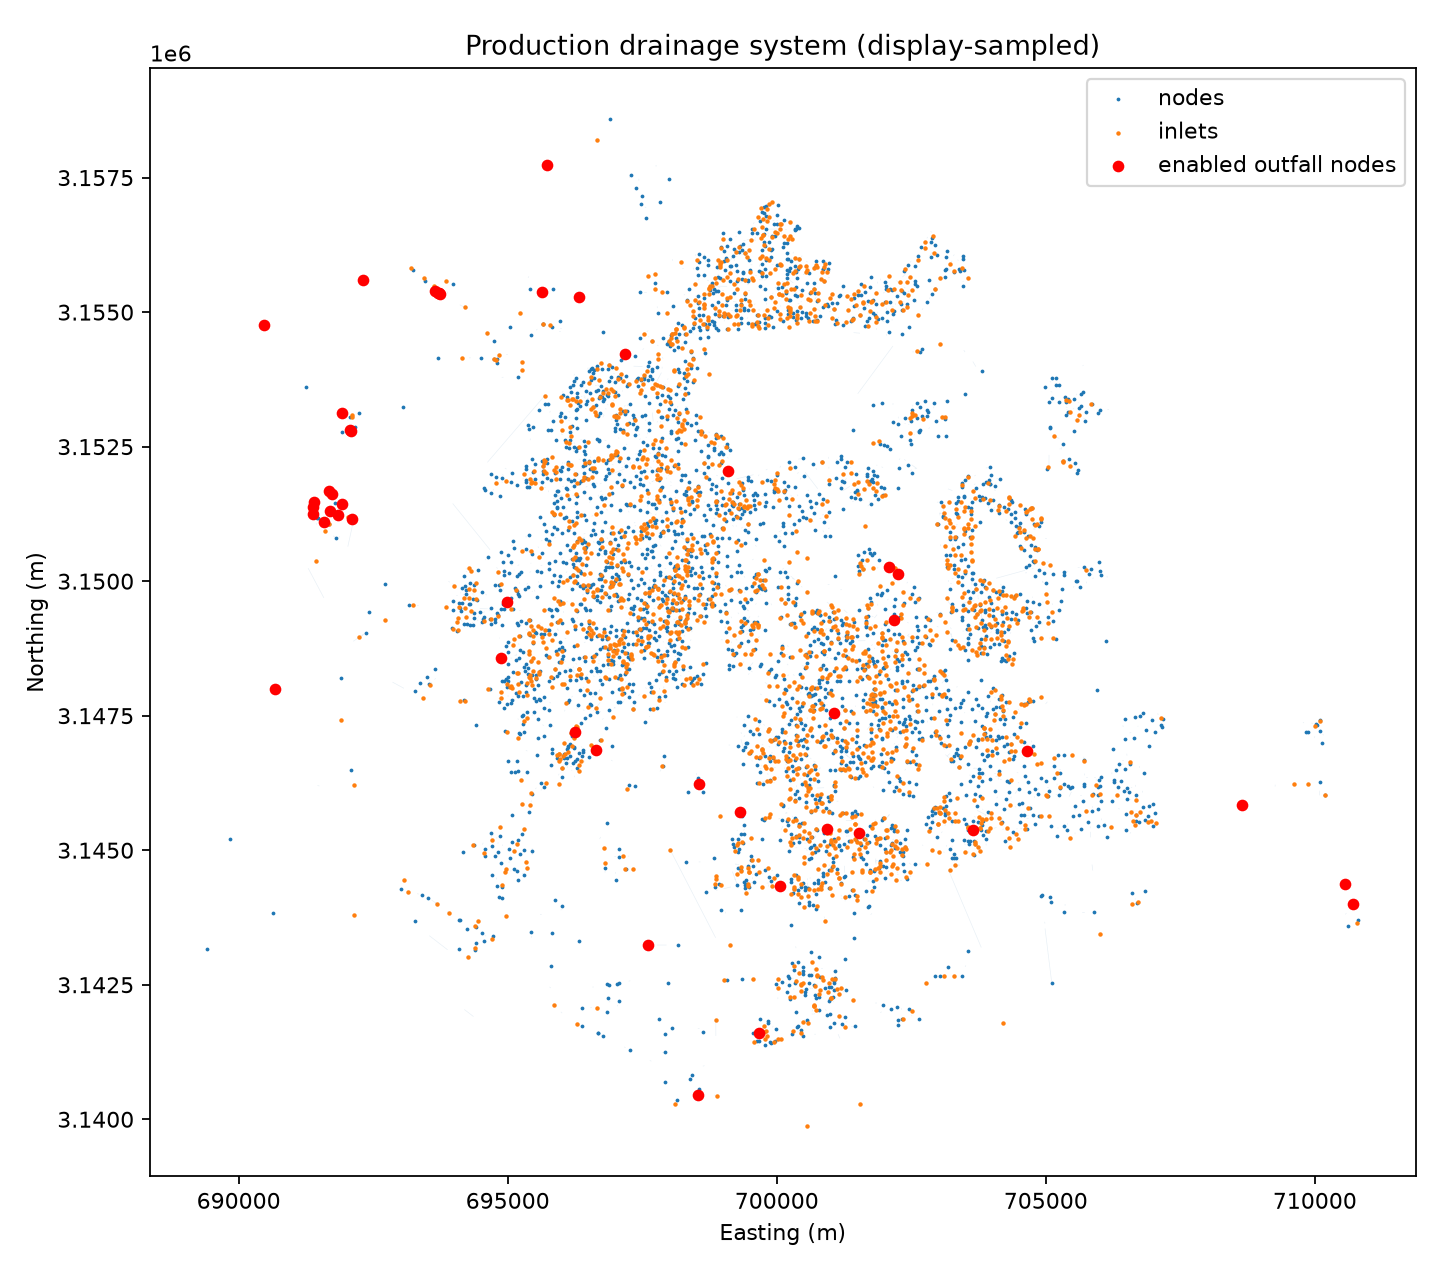
\includegraphics[width=\linewidth]{07_drainage.png}
\caption{Surface-associated drainage network.}
\end{subfigure}
\caption[Production surface mesh and drainage topology.]{The production surface mesh and
drainage topology. Figures are generated directly from the packaged production arrays.}
\label{fig:domain}
\end{figure}

\section{Terrain and resistance}
Centroid bed elevations are finite for all 981,880 triangles, so no runtime terrain filling is used in
the production experiment. The source coordinate reference system is known, but the vertical datum
is not documented. Elevation differences are used by hydrostatic reconstruction and hydraulic heads;
absolute-elevation interpretation must therefore retain this datum limitation. Spatial Manning
coefficients are also present for every triangle, ranging from 0.018 to 0.080 with mean 0.04613 in
the production field. They are active numerical friction parameters, not metadata-only attributes.

\begin{figure}[htbp]
\centering
\begin{subfigure}[t]{0.43\textwidth}
    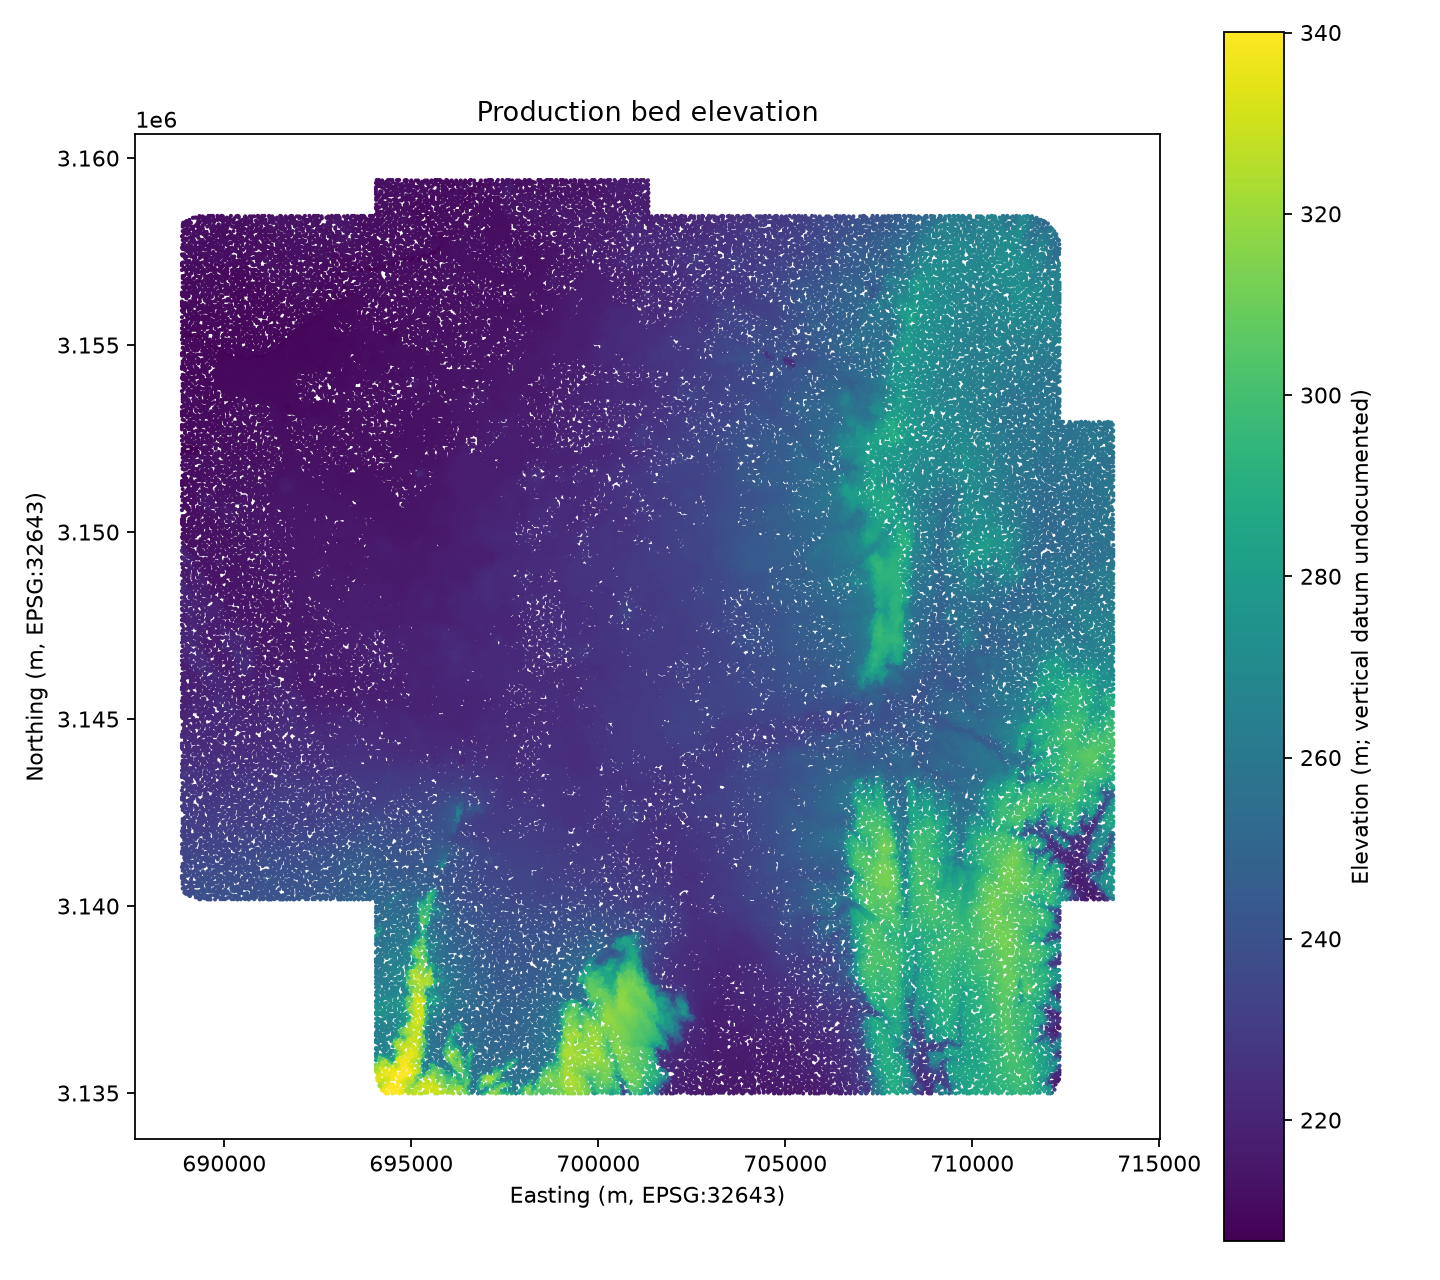
\includegraphics[width=\linewidth]{02_dem.png}
    \caption{Centroid bed elevation.}
\end{subfigure}
\hfill
\begin{subfigure}[t]{0.43\textwidth}
    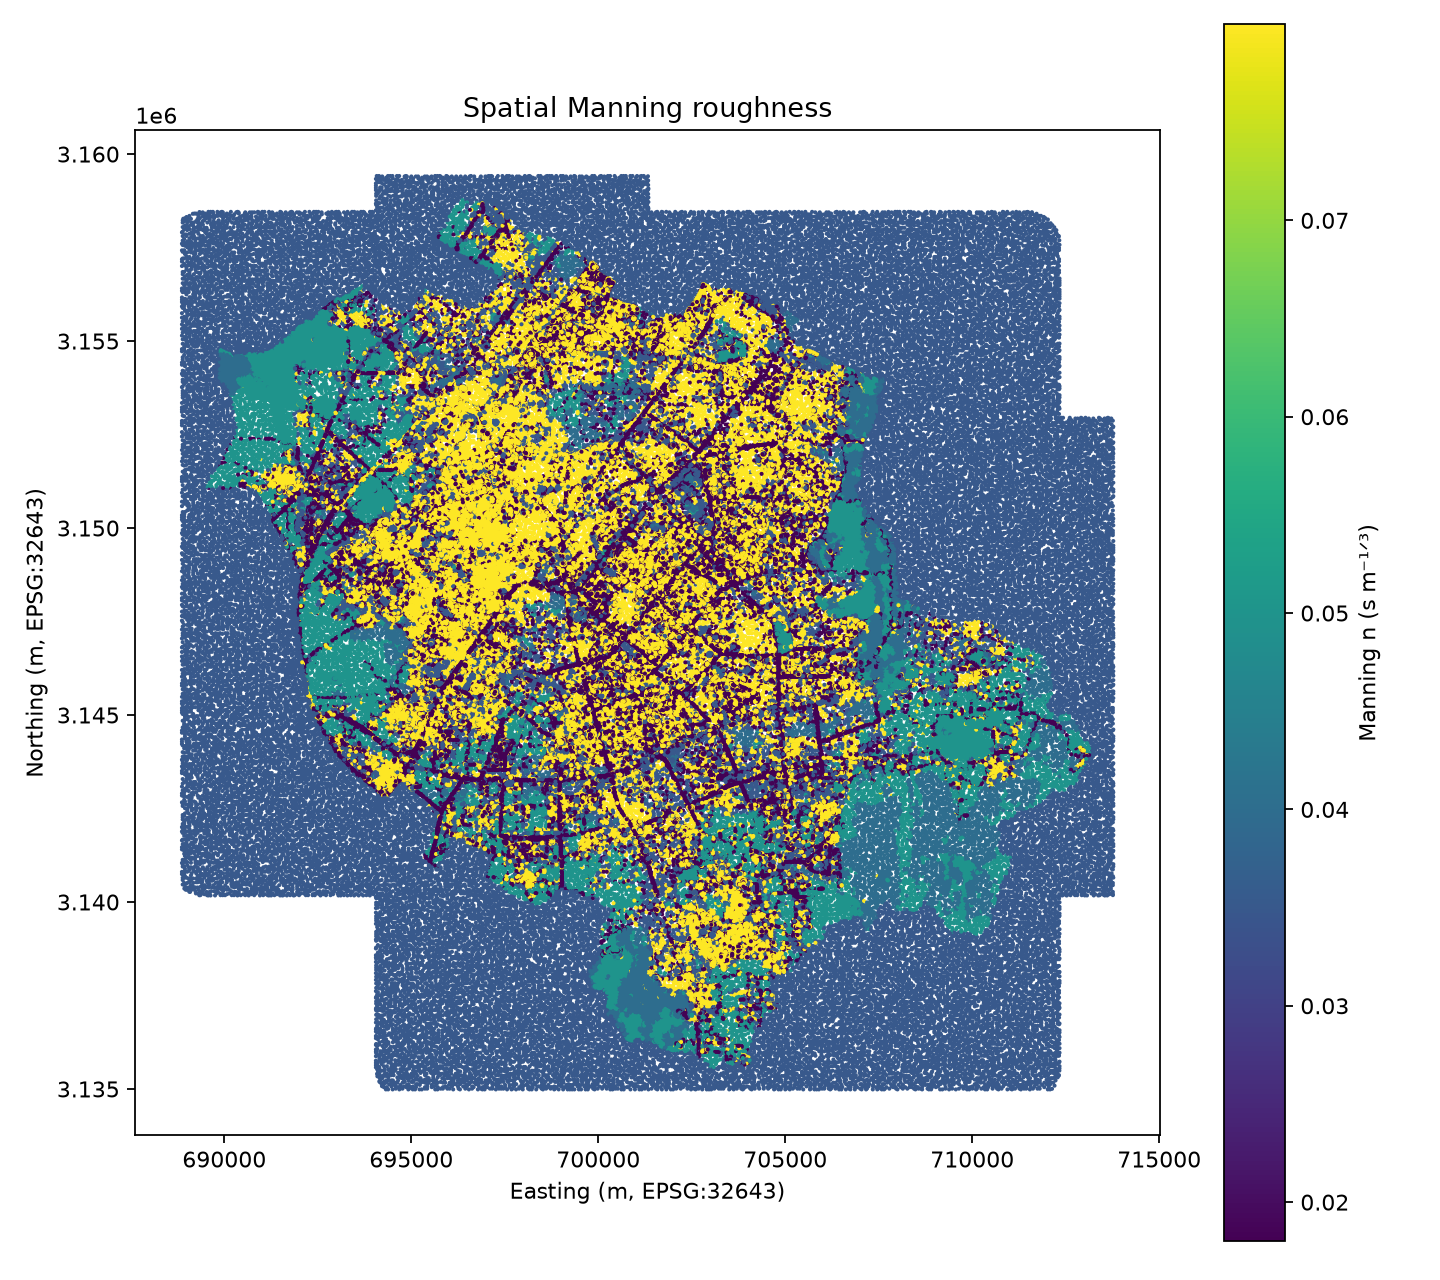
\includegraphics[width=\linewidth]{04_manning.png}
    \caption{Spatial Manning coefficient.}
\end{subfigure}
\caption{Terrain and hydraulic resistance fields used by both production backends.}
\label{fig:terrain_resistance}
\end{figure}



\section{Rainfall, infiltration and boundaries}
The forcing table contains 24 one-hour piecewise-constant intensities whose sum is
\SI{160.09}{\milli\metre}. Rainfall is spatially uniform because the cell multiplier is one,
but losses are spatially heterogeneous through Horton fields. Initial Horton capacity
$f_0$ ranges from 0.0128 to \SI{7.2}{\milli\metre\per\hour}; final capacity $f_c$ ranges
from 0.004 to \SI{2.25}{\milli\metre\per\hour}; the decay coefficient is
\SI{4}{\per\hour}. The boundary subsystem includes an external hydrograph mapped to 150
receiver cells, with a reported peak total flow of \SI{95.1714}{\cubic\metre\per\second}.
These inputs are modelling data and priors; their presence does not by itself constitute
observational validation of the simulated flood.

\begin{figure}[htbp]
\centering
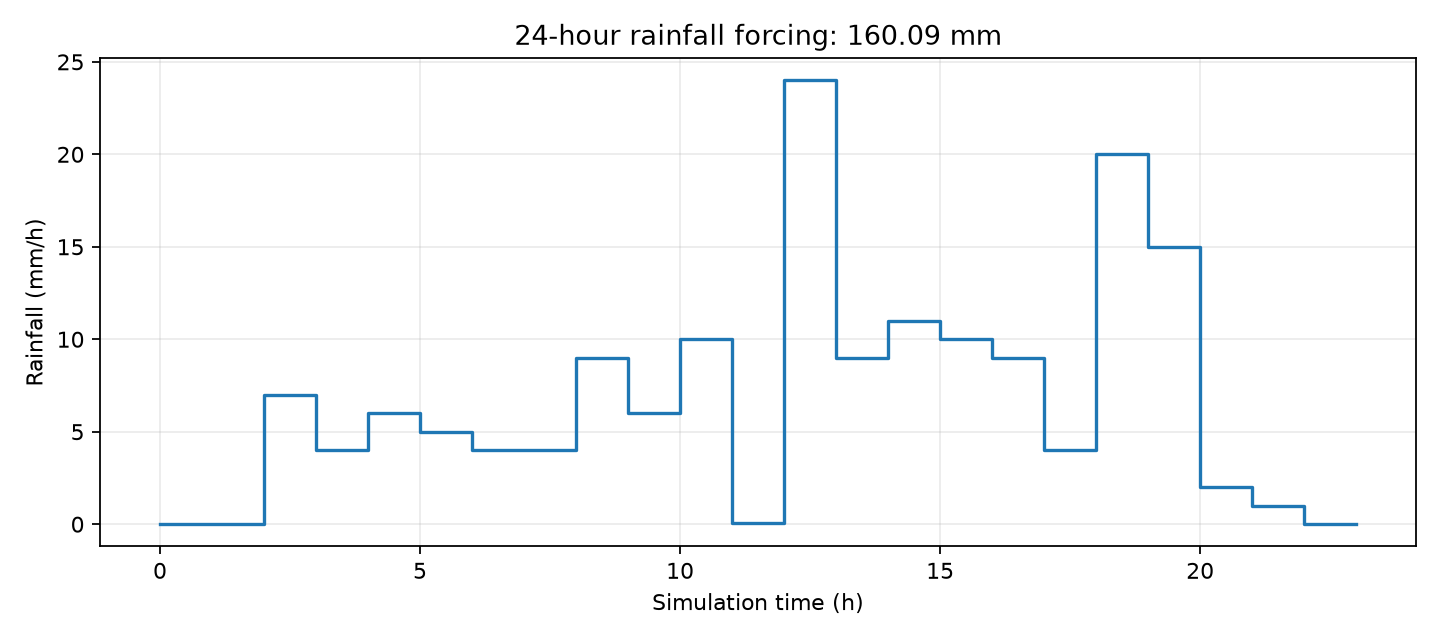
\includegraphics[width=0.70\textwidth]{05_rainfall.png}
\caption[Production rainfall hyetograph.]{The 24-hour production rainfall hyetograph. The event total is
\SI{160.09}{\milli\metre}; intensities are converted from mm h$^{-1}$ to m s$^{-1}$ inside
the model.}
\label{fig:rain}
\end{figure}

\enlargethispage{4\baselineskip}
\section{Drainage representation and provenance}
Surface water may enter 61,317 mapped inlets, move through 139,798 links, leave through 46
enabled outfalls, return through surcharge and interact with 447 recharge records. The
initial surface is dry, while drainage storage is initialized from the approved topology
profile rather than assumed empty. 

\newpage

The package stores source manifests and SHA-256 hashes
for the topology, Horton, recharge, boundary-inflow and rainfall assets. Required topology
fields fail validation when absent; the production runner does not silently create missing
scientific fields.

\section{Input preparation and quality assurance}
The production calculation did not operate directly on loosely related GIS layers. The
source material was transformed into indexed arrays whose dimensions and connectivity agree
with the computational mesh. Triangle centroids and vertex coordinates retain the projected
EPSG:32643 reference, edge records identify their adjacent cells, and each active surface
cell has a finite bed elevation and Manning value. Drainage links refer to valid node
indices, while inlet and recharge records are explicitly mapped to receiving surface cells.
This preprocessing is important because a physically meaningful coefficient attached to the
wrong cell is still a numerically valid array and may otherwise pass simple shape checks.

The executed input path applies progressively stronger checks. First, required filenames and
configuration keys must exist. Second, the loader checks array ranks, lengths, dtypes,
finite values and index ranges. Third, topology summaries compare counts and active area with
the expected production inventory. Finally, hashes preserve the identity of the scientific
assets used by both backends. Missing required topology fields cause a failure instead of a
default value being silently manufactured. The resulting readiness record marked the
production topology as ready and reported no external-inflow snap warnings.

\begin{table}[H]
\centering
\caption[Scientific input traceability.]{Input role, execution representation and completed
quality control.}
\label{tab:inputtrace}
\footnotesize
\begin{tabularx}{\textwidth}{|p{0.19\textwidth}|p{0.24\textwidth}|X|}
\hline
\textbf{Scientific input} & \textbf{Numerical representation} & \textbf{Completed check} \\
\hline\hline
Surface geometry & vertices, triangles, centroids, edges, areas and normals & Dimensions,
connectivity, active mask and domain inventory recorded \\ \hdashline[0.4pt/1.2pt]
Terrain and resistance & one elevation and Manning coefficient per triangle & All 981,880
elevations finite; full spatial roughness field retained \\ \hdashline[0.4pt/1.2pt]
Rainfall and infiltration & hourly intensity series; spatial Horton arrays & Units converted
at the model interface; 24-hour event and parameter ranges recorded \\ \hdashline[0.4pt/1.2pt]
Drainage and recharge & node/link graph, inlet mapping and 447 recharge rows & Node and cell
indices validated; six recharge sources explicitly remapped \\ \hdashline[0.4pt/1.2pt]
Boundary forcing & code-4 exterior edges and 150 hydrograph receivers & Outflow semantics,
receiver count, total hydrograph and spatial snap distances checked \\
\hline
\end{tabularx}
\end{table}

\section{Masks and hydraulic roles}

The archived surface arrays distinguish active cells, buildings and roads. The active mask
determines where the surface equations advance; it contains 817,573 true entries, or 83.266\%
of all triangles. Building and road masks cover 29.028\% and 41.720\% of the triangles,
respectively. These masks provide spatial information used in the construction of hydraulic
properties and domain status, while the production solver directly consumes the resulting
active mask, elevations, roughness and Horton fields.

The boundary geometry is similarly explicit. Inactive neighbours are closed walls, whereas the
34,390 exterior code-4 edges permit outward flux. Historical external inflow is not introduced
by reversing that edge rule; it is added as a separately accounted source to 150 mapped receiver
cells. Keeping these two mechanisms separate makes outward boundary loss and prescribed inflow
independently visible in the mass ledger.

\begin{figure}[H]
    \centering
    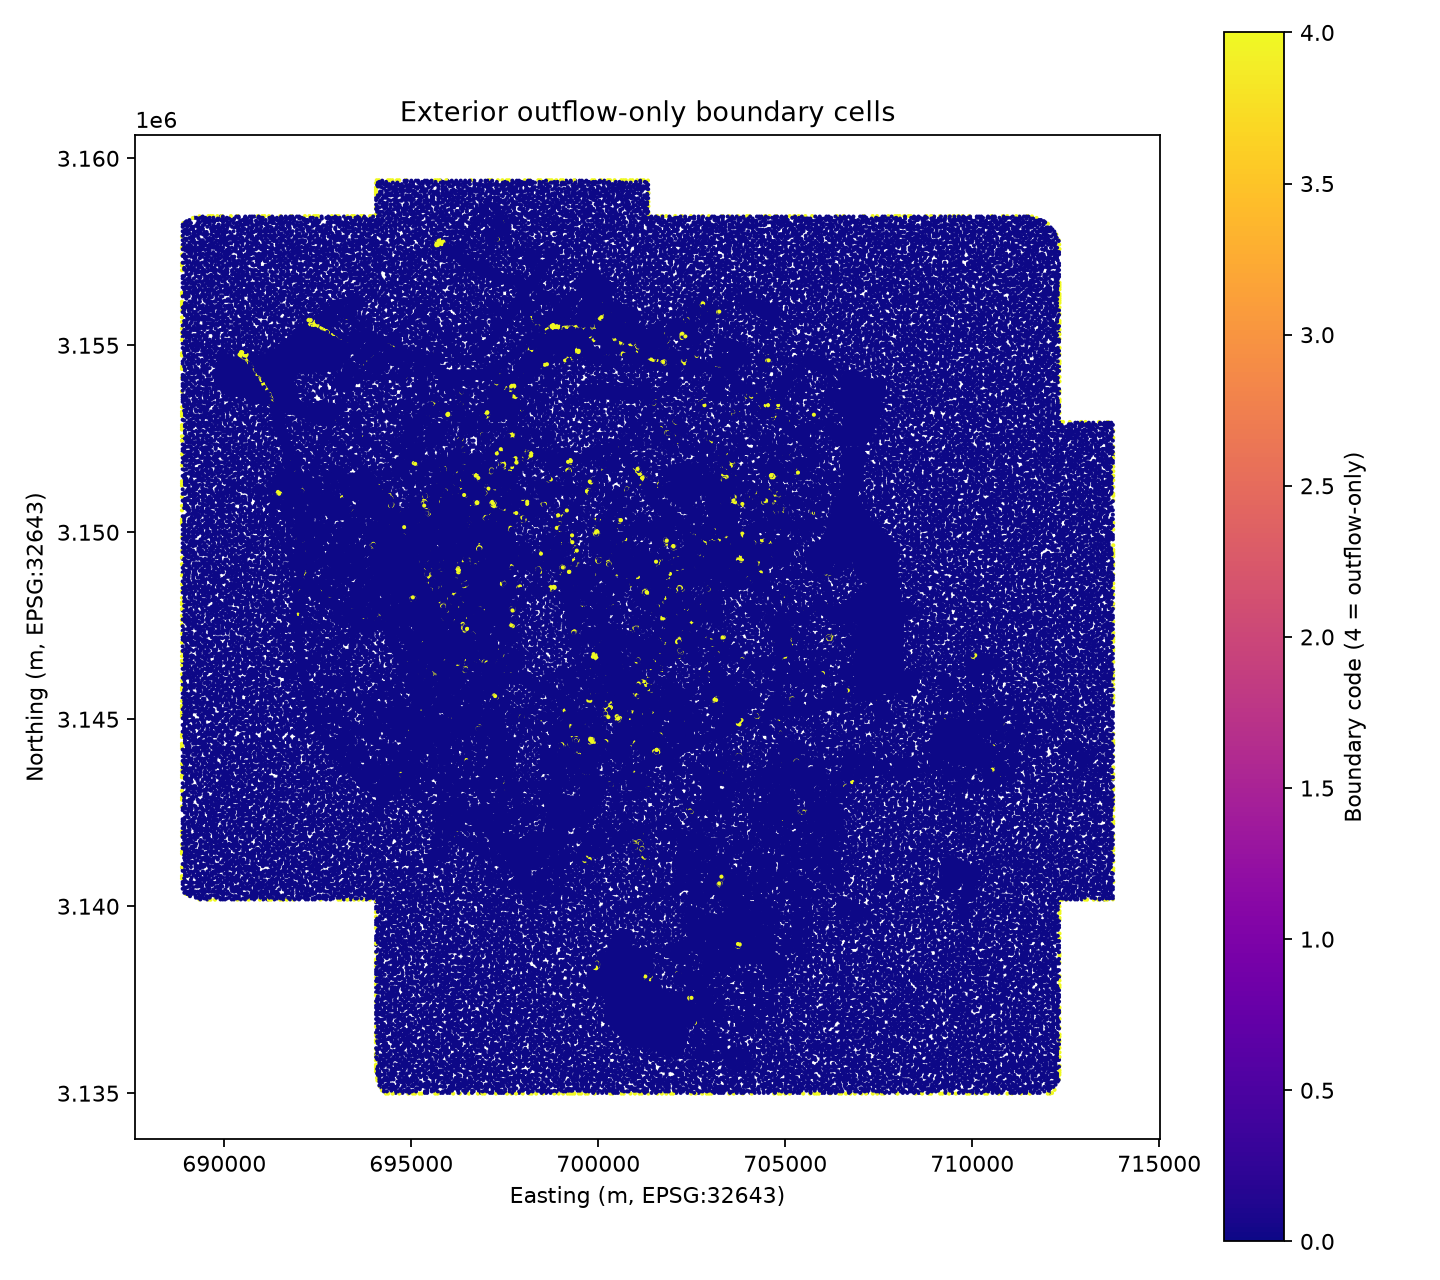
\includegraphics[width=0.54\textwidth]{08_boundaries.png}
    \caption[Production boundary representation.]{Exterior code-4 boundary locations in the
    production domain. Prescribed historical inflow is handled separately at mapped receiver
    cells. \projectsource}
    \label{fig:boundaries}
\end{figure}

% =============================================================================
\chapter{Physical and Numerical Model}\label{chap:physics}
% =============================================================================
\section{Governing equations}
The surface state in each cell is
\begin{equation}
 \bm U=\begin{bmatrix}h&hu&hv\end{bmatrix}^{\mathsf T},
\end{equation}
where $h$ is water depth, $u$ and $v$ are depth-averaged velocities, and $hu,hv$ are
depth-integrated momenta. The conservative two-dimensional shallow-water system is written
in the standard finite-volume conservation form \cite{leveque2002}:
\begin{equation}
 \frac{\partial \bm U}{\partial t}
 +\frac{\partial \bm F(\bm U)}{\partial x}
 +\frac{\partial \bm G(\bm U)}{\partial y}=\bm S,
 \label{eq:swe}
\end{equation}
with
\begin{equation}
 \bm F=\begin{bmatrix}hu\\hu^2+\tfrac12gh^2\\huv\end{bmatrix},\qquad
 \bm G=\begin{bmatrix}hv\\huv\\hv^2+\tfrac12gh^2\end{bmatrix}.
\end{equation}
The source vector contains rainfall, infiltration and exchange contributions to depth,
together with bed and friction effects on momentum. Gravity is
$g=\SI{9.80665}{\metre\per\second\squared}$.

\section{Finite-volume update and HLL flux}
Integrating \cref{eq:swe} over triangular cell $i$ of area $A_i$ gives the explicit update
\begin{equation}
 \bm U_i^{n+1}=\bm U_i^n-
 \frac{\Delta t}{A_i}\sum_{e\in\partial i}L_e\widehat{\bm F}_{e,i}
 +\Delta t\,\bm S_i,
 \label{eq:fvm}
\end{equation}
where $L_e$ is edge length and $\widehat{\bm F}$ is the numerical flux normal to the edge.
For left and right wave-speed estimates $s_L$ and $s_R$, the HLL middle flux is
\begin{equation}
 \widehat{\bm F}_{\mathrm{HLL}}=
 \frac{s_R\bm F_L-s_L\bm F_R+s_Ls_R(\bm U_R-\bm U_L)}{s_R-s_L},
\end{equation}
with the left or right physical flux selected when both waves travel in one direction
\cite{harten1983}. This approximate Riemann solver is local to each edge and therefore maps
well to parallel hardware.

\section{Hydrostatic reconstruction and terrain}
To combine fluxes with discontinuous bed elevation, the interface bed is
$z^*=\max(z_L,z_R)$ and reconstructed depths are
\begin{equation}
 h_L^*=\max(h_L+z_L-z^*,0),\qquad
 h_R^*=\max(h_R+z_R-z^*,0).
\end{equation}
The HLL flux uses these reconstructed depths, while paired pressure corrections
$\tfrac12g(h^2-h^{*2})$ are applied to the two adjacent cells. This Audusse-style
hydrostatic reconstruction supports non-negative depth and lake-at-rest balance
\cite{audusse2004}. Consequently, the DEM and spatially varying elevation are genuine
inputs to the production update.

\section{Wetting, drying, resistance and velocity control}
A minimum depth of $h_{\min}=10^{-5}$ m protects velocity division. Cells below this
threshold have zeroed momenta. Manning resistance is applied semi-implicitly:
\begin{equation}
 (hu,hv)^{n+1}=\frac{(hu,hv)^*}
 {1+\Delta t\,g n^2\lVert\bm u^*\rVert/
        \max(h,h_{\min})^{4/3}},
 \label{eq:manning}
\end{equation}
where $n$ is the spatial roughness coefficient; this resistance convention follows the
standard Manning formulation \cite{chow1959}. A maximum allowed speed of
\SI{5}{\metre\per\second} is subsequently enforced by proportional momentum scaling. The
depth is clipped non-negative after flux and exchange updates.

\section{Rainfall and Horton infiltration}
Rainfall intensity $r(t)$ is evaluated as a one-hour step function and converted to SI
units. For cell multiplier $m_i$, gross rainfall depth added over a step is
\begin{equation}
 \Delta h_{r,i}=r(t)m_i\Delta t.
\end{equation}
Horton infiltration capacity evolves with accumulated wet time $\tau_i$ as
\begin{equation}
 f_i(\tau_i)=f_{c,i}+(f_{0,i}-f_{c,i})e^{-k_i\tau_i},
 \label{eq:horton}
\end{equation}
and actual loss is limited by both $f_i\Delta t$ and available water \cite{horton1933}.
This avoids removing more water than exists in a cell. Momentum is scaled consistently with
remaining depth.

\section{Surface--drainage coupling}
For an inlet linking a surface cell to a drainage node, the implemented exchange follows an
orifice-type head relation
\begin{equation}
 Q_e=C_d A_e\sqrt{2g\lvert H_s-H_n\rvert}\,
      \operatorname{sgn}(H_s-H_n),
\end{equation}
subject to inlet capacity and available-volume constraints. Pipe flow is advanced from
head slope with Manning and minor-loss damping and is bounded by link capacity. Outfall
discharge has the form
\begin{equation}
 Q_o=C_oA_o\sqrt{2g\lvert H_n-H_t\rvert}\,
      \operatorname{sgn}(H_n-H_t),
\end{equation}
then is limited to positive outflow, configured capacity and available node volume.
Excess node storage returns to mapped surface cells as surcharge. Recharge captures water
above a stop depth, stores it subject to capacity, and removes it at a specified recharge
rate.

\section{Boundary conditions, timestep and update order}
Inactive neighbours generate reflective closed-wall states. Exterior code-4 edges allow outflow but
block flux-directed inflow; the approved external hydrograph is added separately to mapped receiver
cells. The stable step satisfies
\begin{equation}
\Delta t =
\min\left[
\Delta t_{\max},
C_{\mathrm{CFL}}
\min_i
\frac{\ell_i}
{\|\mathbf{u}_i\|+\sqrt{g h_i}}
\right],
\qquad
C_{\mathrm{CFL}}=0.85,
\qquad
\Delta t_{\max}=1~\mathrm{s}.
\label{eq:cfl_timestep}
\end{equation}

Each production step follows the same order in both backends: surface flux and friction; rainfall
and Horton loss; velocity limiting; external inflow; inlet exchange; pipe and outfall flow;
overflow return; recharge; and wet-time update. The output schedule produces 25 stored states
over the 24-hour simulation.

\section{Discrete computation sequence}
The ordering of operations is part of the numerical model because nonlinear clipping,
capacity limits and wet--dry decisions do not generally commute. Both backends therefore
use the same staged sequence shown in \cref{tab:update}. Fluxes first move conserved
quantities between adjacent triangles. Rainfall and external inflow add water; infiltration,
outfalls and recharge loss remove or retain it; inlet and surcharge terms exchange water
between the surface and network. The same timestep multiplies all contributions in an
accepted update.

\begin{table}[H]
\centering
\caption{Ordered production update and its conservative or diagnostic role.}
\label{tab:update}
\small
\begin{tabularx}{\textwidth}{|c|p{0.29\textwidth}|X|}
\hline
\textbf{Stage} & \textbf{Operation} & \textbf{Role in the update} \\
\hline\hline
1 & Hydrostatic HLL surface flux & Transfers depth and momentum across mesh edges and
applies balanced bed-pressure corrections \\ \hdashline[0.4pt/1.2pt]
2 & Manning friction and speed control & Damps momentum, protects dry cells and enforces
the registered velocity ceiling \\ \hdashline[0.4pt/1.2pt]
3 & Rainfall and Horton infiltration & Adds gross precipitation and removes only the
capacity- and availability-limited infiltration depth \\ \hdashline[0.4pt/1.2pt]
4 & External inflow and inlet exchange & Applies prescribed surface input and transfers
available water between mapped surface cells and drainage nodes \\ \hdashline[0.4pt/1.2pt]
5 & Pipes, outfalls and surcharge & Advances network conveyance, discharges at enabled
outfalls and returns excess storage to the surface \\ \hdashline[0.4pt/1.2pt]
6 & Recharge and diagnostics & Updates recharge storage and loss, wet time, extrema,
cumulative ledgers and scheduled snapshots \\
\hline
\end{tabularx}
\end{table}

The adaptive timestep is recomputed from the current hydraulic state and reused only under
the configured safety policy.

\section{System mass ledger}
For any accepted time interval, the diagnostic balance can be written generically as
\begin{equation}
 R_M=V_{s,0}+V_{n,0}+\sum V_{\mathrm{in}}
       -\sum V_{\mathrm{loss}}-V_{s,f}-V_{n,f}-V_{r,f},
 \label{eq:massledger}
\end{equation}
where $V_s$, $V_n$ and $V_r$ are surface, drainage-node and explicitly retained recharge
storage. Inputs include rainfall and prescribed external inflow. Losses include
infiltration, net outward boundary transfer, outfall discharge and recharge removal.
Surface-to-network capture and surcharge are internal exchanges: they are recorded for
diagnosis but cancel when the complete coupled system is considered. The solver convention
records boundary net flux as positive inward and negative outward, so sign conversion is
required when it is placed in the loss column of a presentation table.

The residual $R_M$ measures numerical closure of the registered ledger; it is not an
unmodelled physical discharge. Its ratio uses the package's common comparison denominator.
The JAX report provides both a CuPy-compatible residual, which omits final recharge storage
to match the reference ledger, and a complete residual that includes it. This dual reporting
preserves a like-for-like regression check without discarding the more complete accounting.

% =============================================================================
\chapter{GPU Implementation Architecture}\label{chap:gpu}
% =============================================================================
\section{One model, two accelerator paths}
The comparison is designed around mathematical equivalence, not identical source code.
Both paths load the same hashed arrays and preserve state ordering, units, single-precision
surface variables, source sequence and output schedule. The state is represented by
structure-of-arrays fields for $h$, $hu$, $hv$, wet time, node storage, link discharge and
recharge storage. Edge-local work and indexed accumulation dominate the surface update;
graph-local work dominates drainage exchange.

\section{CuPy/CUDA implementation}
CuPy exposes NumPy-compatible arrays on CUDA devices \cite{cupy}. The reference backend
uses fused custom CUDA production kernels for surface and drainage operations, reducing
Python dispatch and avoiding host--device transfers during stepping. The recorded
implementation identifier is \texttt{gurugram\_flood\_backend\_fused\_cuda}. Device arrays
remain on CUDA device 0; only final products and diagnostics are transferred for storage.
This backend serves as the numerical reference for parity, not as physical truth.

\section{JAX/XLA implementation}

JAX traces pure array functions and lowers them through XLA \cite{jax}. The production path uses
immutable named state tuples, scatter-add reductions for edge and network accumulation, and
a compiled \texttt{while\_loop}. Inactive tail iterations are avoided. Compilation and execution
are synchronized before timing. The first compiled output chunk includes compilation and
execution, while subsequent chunk runtimes represent the already compiled path. The
implementation identifier is \texttt{hybrid\_flood\_v2\_jax\_v1\_parity}.

\section{Role of PyTorch}
PyTorch supports imperative tensor computation and CUDA acceleration \cite{pytorch}. It
was available in the production environment and its CUDA capability was confirmed, but it
was not an execution backend for the final complete-domain experiment. The implementations
timed here are CuPy and JAX. Therefore, no PyTorch runtime is placed in the benchmark table and no
CuPy--PyTorch or JAX--PyTorch speed claim is made.

\section{Execution environment}
\begin{table}[H]
\centering
\caption[Production GPU and software environment.]{Recorded production GPU and software
environment. \projectsource}
\label{tab:env}
\small
\begin{tabularx}{0.92\textwidth}{|l|X|}
\hline
\textbf{Item} & \textbf{Recorded value} \\
\hline\hline
GPU & NVIDIA RTX PRO 4000 Blackwell, 24,467 MiB \\ \hdashline[0.4pt/1.2pt]
Driver / CuPy CUDA runtime & 595.84 / 13.2 \\ \hdashline[0.4pt/1.2pt]
Python & 3.12.14 \\ \hdashline[0.4pt/1.2pt]
CuPy / NumPy & 14.1.1 / 2.5.1 \\ \hdashline[0.4pt/1.2pt]
JAX / jaxlib & 0.10.2 / 0.10.2 \\ \hdashline[0.4pt/1.2pt]
PyTorch & 2.13.0+cu130; CUDA availability confirmed \\ \hdashline[0.4pt/1.2pt]
Selected devices & CuPy device 0; JAX \texttt{cuda:0} \\ \hdashline[0.4pt/1.2pt]
Fallback & CPU fallback false \\ \hdashline[0.4pt/1.2pt]
Primary surface precision & float32 \\
\hline
\end{tabularx}
\end{table}

The environment record is essential because compiler, driver and GPU architecture can
affect both floating-point ordering and performance. The report therefore interprets the
timings as results for this specific hardware--software configuration rather than universal
framework rankings.

\section{Parallel work and device-resident data}
The surface update exposes one large parallel problem over 1,490,015 edges. Each edge reads
the states and bed elevations of its adjacent triangles, constructs wet--dry-safe interface
states, evaluates wave speeds and produces flux contributions. Those contributions must
then be accumulated into as many as 981,880 cell states. The drainage calculation has a
corresponding graph structure over 139,798 links and 118,768 nodes, followed by sparse
surface--network exchanges at mapped inlets. These indexed accumulations, rather than the
three-component state vector alone, are the principal implementation challenge.

Both implementations store major fields as separate contiguous arrays. This
structure-of-arrays organisation lets adjacent GPU threads read the same physical quantity
for different edges or cells and avoids repeatedly moving structured Python objects. Static
geometry, terrain, coefficients and connectivity are uploaded once; evolving depth,
momentum, wet time and network storage remain device resident through the timestep loop.
Only scheduled results and scalar diagnostics cross the device boundary. For a single
depth-history array alone, 25 float32 states over 981,880 cells represent 24,547,000 finite
values, approximately 93.6 MiB before archive compression.

CuPy expresses the production-critical work through fused CUDA kernels and explicit device
arrays. JAX represents the corresponding operations as traceable array functions, uses
scatter reductions for indexed contributions and places the time loop inside a compiled XLA
control-flow operation. These are different execution strategies for the same staged
calculation. Numerical parity is consequently judged on physical outputs and ledgers, not
on kernel count or identical floating-point instruction order.

\section{Compilation, synchronization and output boundaries}
GPU launches are asynchronous with respect to the host unless a result is explicitly
synchronized. The recorded timing path therefore waits for accelerator completion before
accepting a runtime. JAX compilation is also separated conceptually from steady execution:
the first output chunk records compilation together with execution, and the remaining
chunks use the compiled path.

Hourly output targets do not replace the adaptive solver clock. The solver advances with
subsecond-to-one-second steps and stores the first state after one second followed by requested
hourly targets through 86,400 seconds. Recording this offset prevents spatial fields from being
compared as though their timestamps were mathematically exact and identical.

\begin{table}[H]
\centering
\caption[Backend correspondence in the production calculation.]{Backend correspondence for
the same numerical responsibilities.}
\label{tab:backendmap}
\footnotesize
\begin{tabularx}{\textwidth}{|p{0.22\textwidth}|p{0.27\textwidth}|p{0.27\textwidth}|X|}
\hline
\textbf{Responsibility} & \textbf{CuPy/CUDA path} & \textbf{JAX/XLA path} &
\textbf{Required agreement} \\
\hline\hline
Surface state & device float32 arrays & immutable float32 array state & cell order, units and
initial values \\ \hdashline[0.4pt/1.2pt]
Edge accumulation & fused CUDA kernels & XLA scatter reductions & conservative contribution
to each adjacent cell \\ \hdashline[0.4pt/1.2pt]
Network state & device node/link arrays & compiled named state tuple & topology, capacities
and exchange ordering \\ \hdashline[0.4pt/1.2pt]
Time integration & host-controlled GPU kernels & compiled XLA while loop & CFL rule,
maximum step and output targets \\ \hdashline[0.4pt/1.2pt]
Acceptance & reference products and ledger & candidate products and ledger & all eight
predefined parity gates \\
\hline
\end{tabularx}
\end{table}

% =============================================================================
\chapter{Verification and Experimental Methodology}\label{chap:method}
% =============================================================================
\section{Evidence hierarchy}
Three forms of evidence are kept separate. Software verification asks whether tests and
invariants pass. Numerical verification asks whether two implementations of the same model
agree within registered tolerances. Physical validation asks whether model predictions agree
with observations. The first two are available; the third is not. ANUGA adds an independent
numerical reference on compatible small cases but cannot replace observations.

\section{Production experiment}
Both backends ran the same \SI{24}{\hour} event with \SI{160.09}{\milli\metre} accumulated
rainfall, dry surface initial conditions, topology-defined drainage storage, CFL 0.85,
maximum timestep \SI{1}{\second}, maximum speed \SI{5}{\metre\per\second}, float32 surface
fields and hourly outputs. CuPy was treated as the reference implementation and JAX as the
candidate. This designation defines the direction of errors; it does not imply that CuPy is
an observation.

\section{Parity metrics and acceptance gates}
For valid cells $i=1,\dots,N$, depth error is summarized by
\begin{equation}
 \operatorname{RMSE}_h=\sqrt{\frac1N\sum_i(h_i^{J}-h_i^{C})^2},\qquad
 \operatorname{MAE}_h=\frac1N\sum_i\lvert h_i^{J}-h_i^{C}\rvert.
\end{equation}
With wet sets $W_C$ and $W_J$ defined at the registered threshold, flood-extent overlap is
\begin{equation}
 \operatorname{CSI}=\frac{\lvert W_C\cap W_J\rvert}
 {\lvert W_C\cup W_J\rvert}.
\end{equation}
Relative surface-volume error, maximum-depth error, snapshot-time alignment and source--sink
ledger differences complete the gates. The acceptance limits were fixed before interpreting the comparison; their observed values are reported later with the production parity results \cref{tab:gates}.

\section{Repeatability protocol}
A second independent 24-hour run was compared with run A for each backend using the existing
criteria: depth RMSE at most \SI{0.05}{\metre}, minimum CSI at least 0.95, and snapshot
offset at most \SI{1}{\second}. Archive identity was evaluated separately. This distinction
prevents scientifically acceptable floating-point differences from being incorrectly
reported as bitwise determinism.

\section{Performance protocol}
The completed repeated timing experiment is a secondary, identical 60-minute production
workload. Each backend completed three warm-ups and ten synchronized measurements on the
same device, and every measured output passed its correctness check. Mean, median, range,
population standard deviation, interquartile range and coefficient of variation were
computed from raw measurements. The longer official 24-hour repeated benchmark was stopped
after 10 CuPy and 3 JAX measurements; it therefore provides no official backend ratio and is
not merged with the complete secondary benchmark.

\section{Controls against an invalid comparison}
The comparison was constrained at four levels. At the input level, both implementations
loaded the same topology, terrain, roughness, infiltration, rainfall, recharge, drainage and
boundary assets; manifests and hashes preserve their identity. At the model level, the state
variables, physical constants, wet threshold, source ordering, CFL coefficient, maximum
timestep and output targets were matched. At the execution level, both backends selected
\texttt{cuda:0}, recorded GPU status and prohibited CPU fallback. At the evaluation level,
the parity limits existed before the final interpretation and were applied to every hourly
state rather than only the final map.

CuPy was called the numerical reference because the JAX path was designed to reproduce its
production sequence. This is a software-comparison convention, not an assumption that CuPy
is exact. Errors are consequently signed or labelled as JAX relative to CuPy, while physical
accuracy remains unassessed. The same distinction applies to mass balance: the residual
regression gate detects whether JAX materially worsens the compatible CuPy ledger, whereas
the complete JAX ledger separately accounts for ending recharge storage.


\section{Software verification and package audit}
The final software check collected 148 tests. Of these, 111 passed, 37 were explicitly
skipped, and none failed or raised an error. The run completed in 10.58 s with two warnings.
Skipped tests were classified as outside the final production scope or as requiring the
opposite hardware environment; they were not counted as passes. The result therefore reports both
the successful executable baseline and the exact portion that was not exercised.

\begin{table}[H]
\centering
\caption[Final automated-test outcome.]{Final automated-test outcome and interpretation.}
\label{tab:tests}
\small
\begin{tabular}{|l|r|l|}
\hline
\textbf{Outcome} & \textbf{Count} & \textbf{Interpretation} \\
\hline\hline
Collected & 148 & Total discovered by the test runner \\ \hdashline[0.4pt/1.2pt]
Passed & 111 & Executed successfully \\ \hdashline[0.4pt/1.2pt]
Explicitly skipped & 37 & Excluded-scope or opposite-hardware classification \\ \hdashline[0.4pt/1.2pt]
Failed / errors & 0 / 0 & No failing test or collection/runtime error \\ \hdashline[0.4pt/1.2pt]
Warnings / runtime & 2 / 10.58 s & Preserved runner diagnostics \\
\hline
\end{tabular}
\end{table}

The semantic package audit checked that required reports, machine-readable tables, simulation
archives, figures, environment records and reproduction material were present and mutually
consistent. SHA-256 verification passed. These controls establish provenance: they do not improve
a numerical score, but they identify the evidence supporting each reported result.

% =============================================================================
\chapter{Production Simulation Results}\label{chap:results}
% =============================================================================
\section{Surface and network response}
The two 24-hour runs produced closely aligned domain-scale responses. CuPy used 321,645
timesteps and JAX used 321,640. The domain-wide maximum depths were
\SI{9.414836884}{\metre} and \SI{9.414829254}{\metre}, respectively, while the final numbers
of cells deeper than \SI{0.05}{\metre} were 129,187 and 129,180. The extreme maximum is a
local model value and should not be interpreted as a typical city depth or as a measured
water level.

\begin{table}[H]
\centering
\caption[Principal 24-hour production outputs.]{Principal 24-hour production outputs.}
\label{tab:production}
\small
\begin{tabular}{|l|r|r|}
\hline
\textbf{Quantity} & \textbf{CuPy} & \textbf{JAX} \\
\hline\hline
Solver timesteps & 321,645 & 321,640 \\ \hdashline[0.4pt/1.2pt]
Recorded solver runtime (s) & 430.467 & 451.865 \\ \hdashline[0.4pt/1.2pt]
Maximum depth (m) & 9.414836884 & 9.414829254 \\ \hdashline[0.4pt/1.2pt]
Wet triangles at 0.05 m & 129,187 & 129,180 \\ \hdashline[0.4pt/1.2pt]
Final surface volume (m$^3$) & 23,377,569.249 & 23,375,823.126 \\ \hdashline[0.4pt/1.2pt]
Final node volume (m$^3$) & 420,425.063 & 420,421.469 \\ \hdashline[0.4pt/1.2pt]
Rainfall input (m$^3$) & 47,701,360.545 & 47,701,532.000 \\ \hdashline[0.4pt/1.2pt]
Infiltration loss (m$^3$) & 4,545,656.989 & 4,545,672.500 \\ \hdashline[0.4pt/1.2pt]
Outfall discharge (m$^3$) & 1,060,887.868 & 1,060,836.750 \\
\hline
\end{tabular}
\end{table}

\section{Preserved state and diagnostic products}
The production archives retain more than a final depth map. Each backend stores depth and
speed histories with shape $25\times981{,}880$, final momentum components, event maxima,
surface masks, terrain, coordinates and mesh connectivity. Network products include a
$25\times118{,}768$ node-volume history and final discharge for all 139,798 links. Every
entry of the principal history arrays is finite. This output design supports temporal,
spatial and conservation checks from the same run rather than requiring the solver to be
executed again for each figure.

\begin{table}[H]
\centering
\caption{Selected preserved arrays from the CuPy production archive; the JAX archive has corresponding fields.}
\label{tab:arrays}
\footnotesize
\begin{tabularx}{\textwidth}{|p{0.29\textwidth}|p{0.20\textwidth}|p{0.12\textwidth}|X|}
\hline
\textbf{Array} & \textbf{Shape} & \textbf{Units} & \textbf{Recorded range or role} \\
\hline\hline
Depth snapshots & $25\times981{,}880$ & m & 24,547,000 finite values; event maximum
9.414837 m \\ \hdashline[0.4pt/1.2pt]
Speed snapshots & $25\times981{,}880$ & m s$^{-1}$ & event maximum 1.712713 m s$^{-1}$ \\
\hdashline[0.4pt/1.2pt]
Drainage-node volume snapshots & $25\times118{,}768$ & m$^3$ & temporal network storage
for every node \\ \hdashline[0.4pt/1.2pt]
Final $h$, $hu$, $hv$ & $981{,}880$ each & m; m$^2$ s$^{-1}$ & complete final conserved
surface state \\ \hdashline[0.4pt/1.2pt]
Final link flow & $139{,}798$ & m$^3$ s$^{-1}$ & $-1.56136$ to 3.40805 m$^3$ s$^{-1}$ \\
\hdashline[0.4pt/1.2pt]
Geometry and masks & mesh-dependent & m / indices & coordinates, triangles, terrain,
active, road and building context \\
\hline
\end{tabularx}
\end{table}

The tiny CuPy minimum depth in the full history, $-8.73\times10^{-11}$ m, is far below the
registered $-10^{-7}$ m non-negativity tolerance and the final minimum is approximately
$-5.68\times10^{-14}$ m. JAX stored non-negative depths. These values are retained rather
than rounded away because they document float32 numerical behaviour at nominally dry cells.
They do not represent physically negative water depth.

\begin{figure}[htbp]
\centering
\begin{subfigure}[t]{0.49\textwidth}
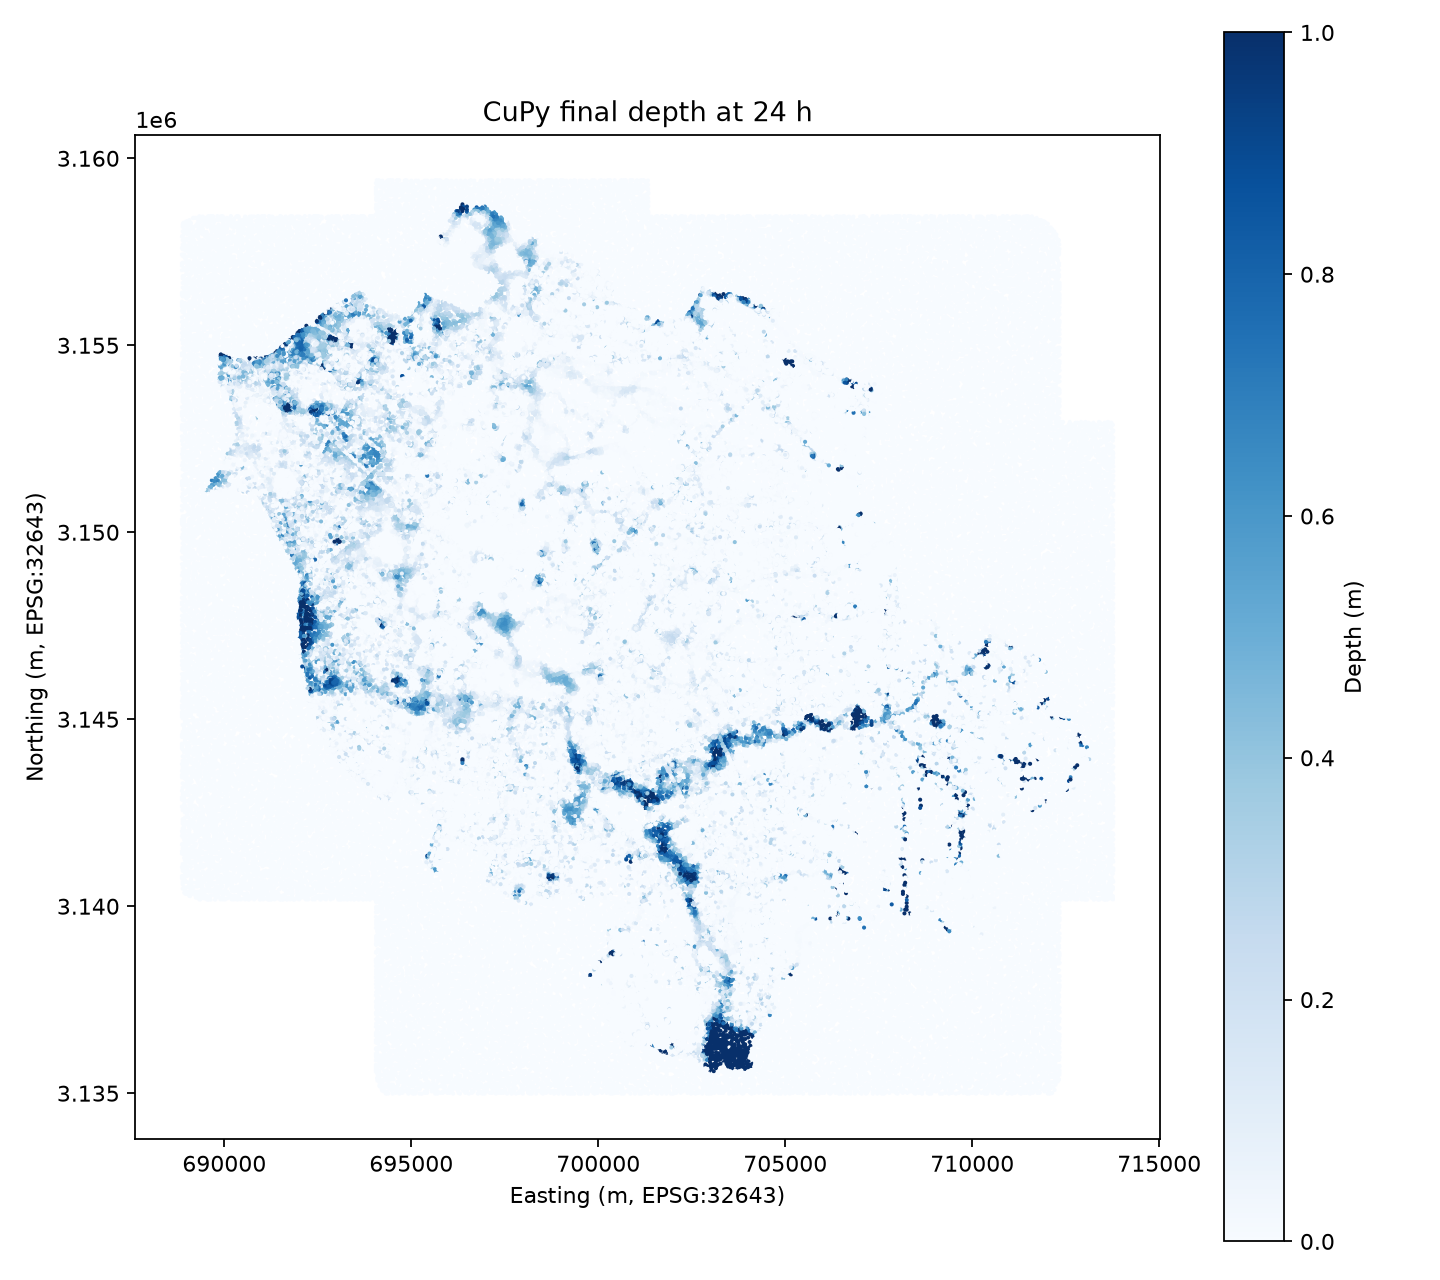
\includegraphics[width=\linewidth]{09_final_depth_cupy.png}
\caption{CuPy final depth.}
\end{subfigure}\hfill
\begin{subfigure}[t]{0.49\textwidth}
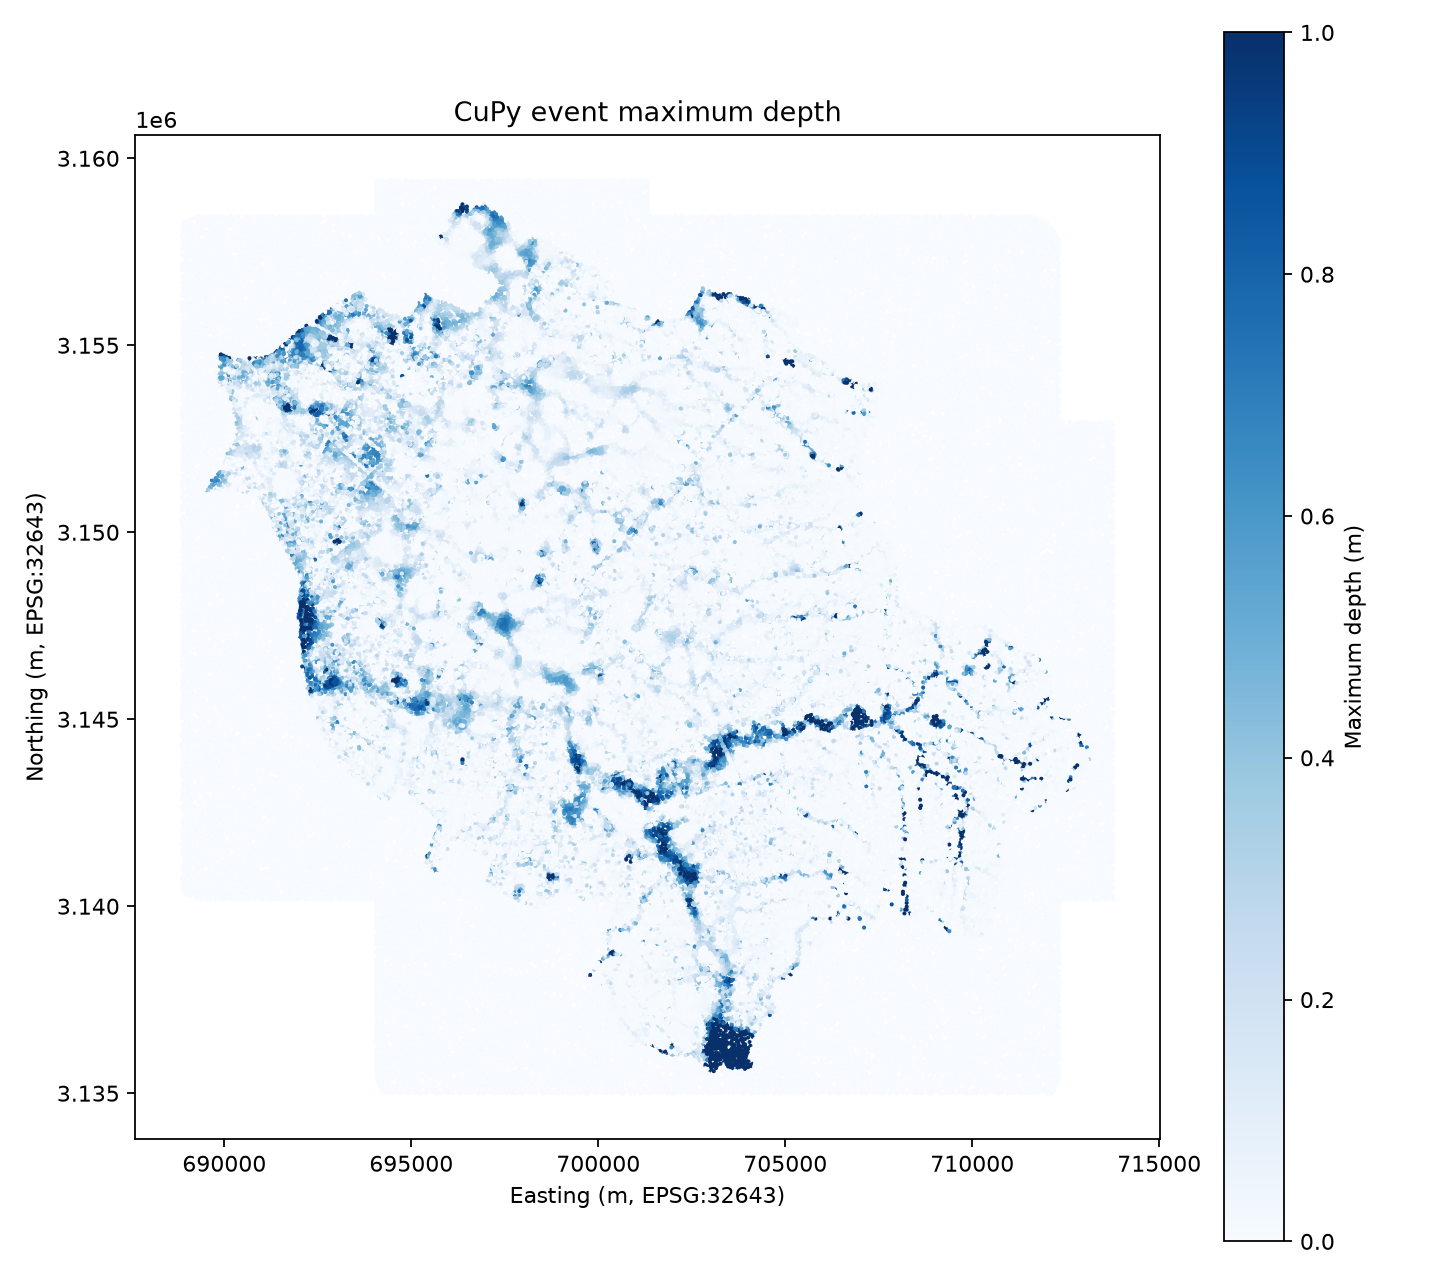
\includegraphics[width=\linewidth]{10_maximum_depth_cupy.png}
\caption{CuPy maximum depth over 24 h.}
\end{subfigure}
\caption[Production surface-water results.]{Production surface-water results. These maps
are model outputs and have not been validated against observed inundation.}
\label{fig:depth}
\end{figure}

\section{Wet extent and timing}
The wet-area threshold for production summaries is \SI{0.05}{\metre}. Final wet-cell counts
differed by seven triangles, consistent with the final CSI of 0.999590. Arrival and duration
products were derived from the 25 stored states and therefore have hourly temporal
resolution; they must not be interpreted as minute-scale timing observations.

\begin{figure}[htbp]
\centering
\begin{subfigure}[t]{0.49\textwidth}
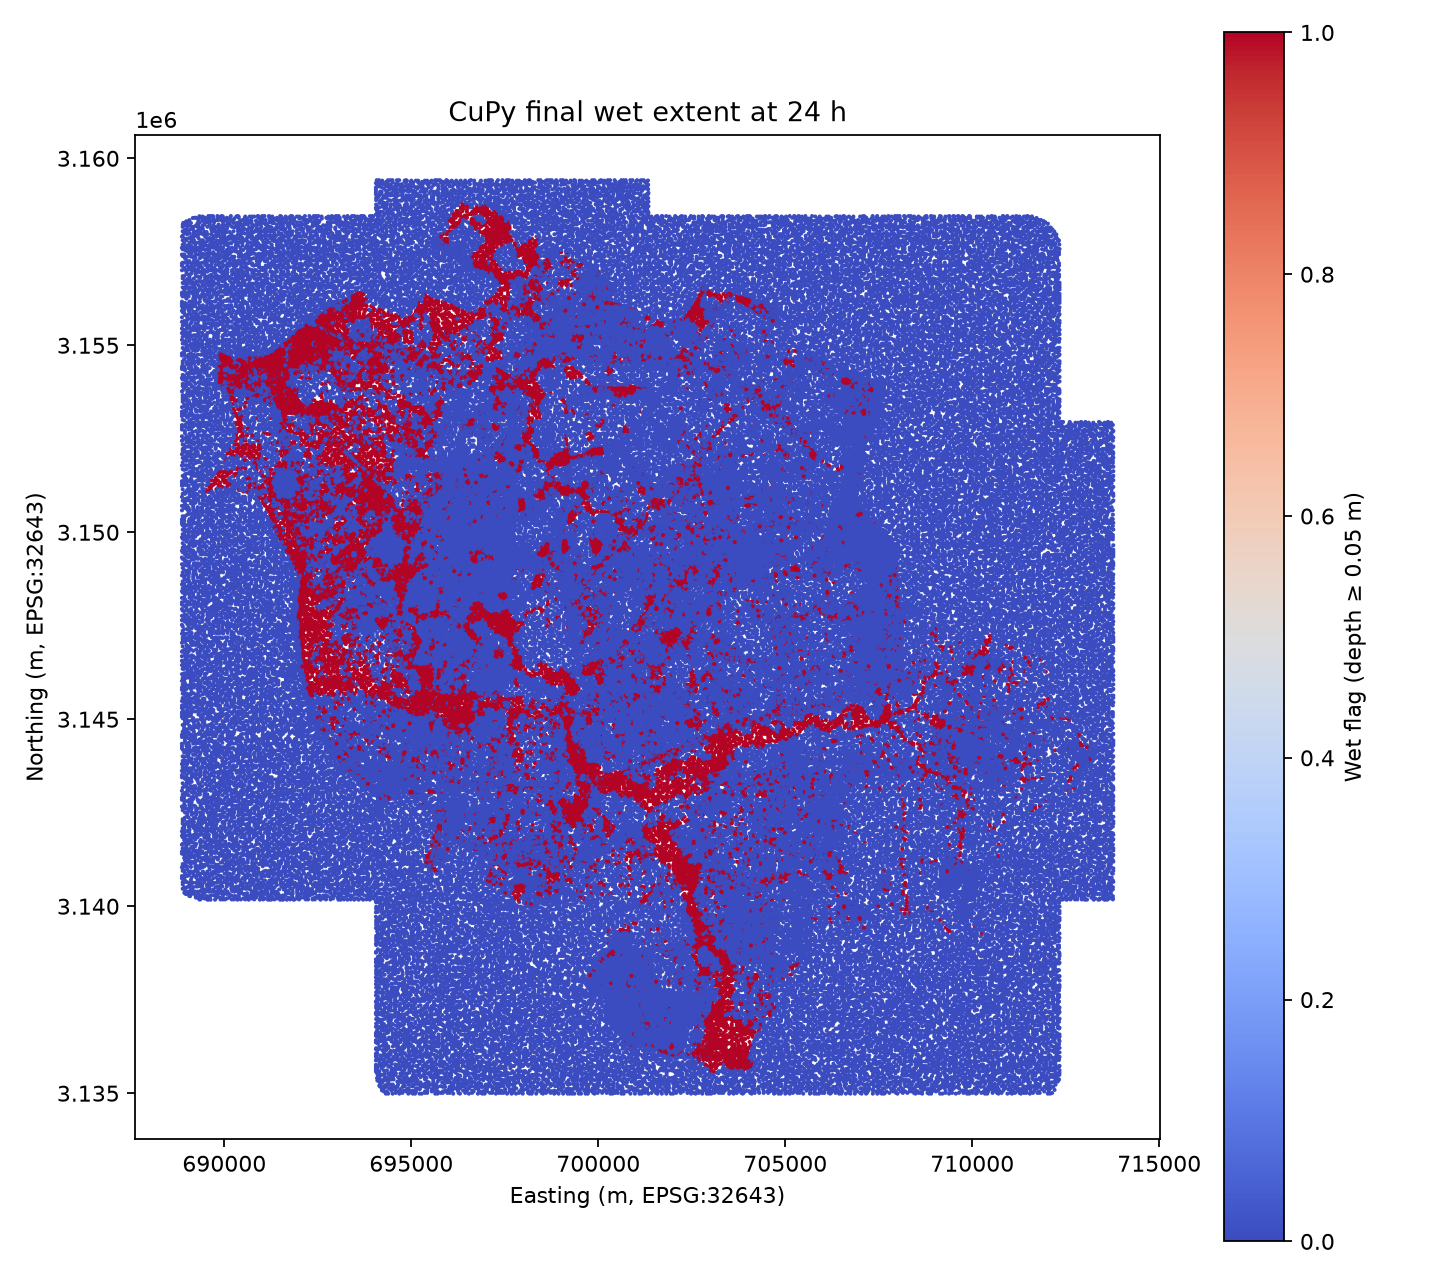
\includegraphics[width=\linewidth]{11_wet_extent.png}
\caption{Wet extent through the event.}
\end{subfigure}\hfill
\begin{subfigure}[t]{0.49\textwidth}
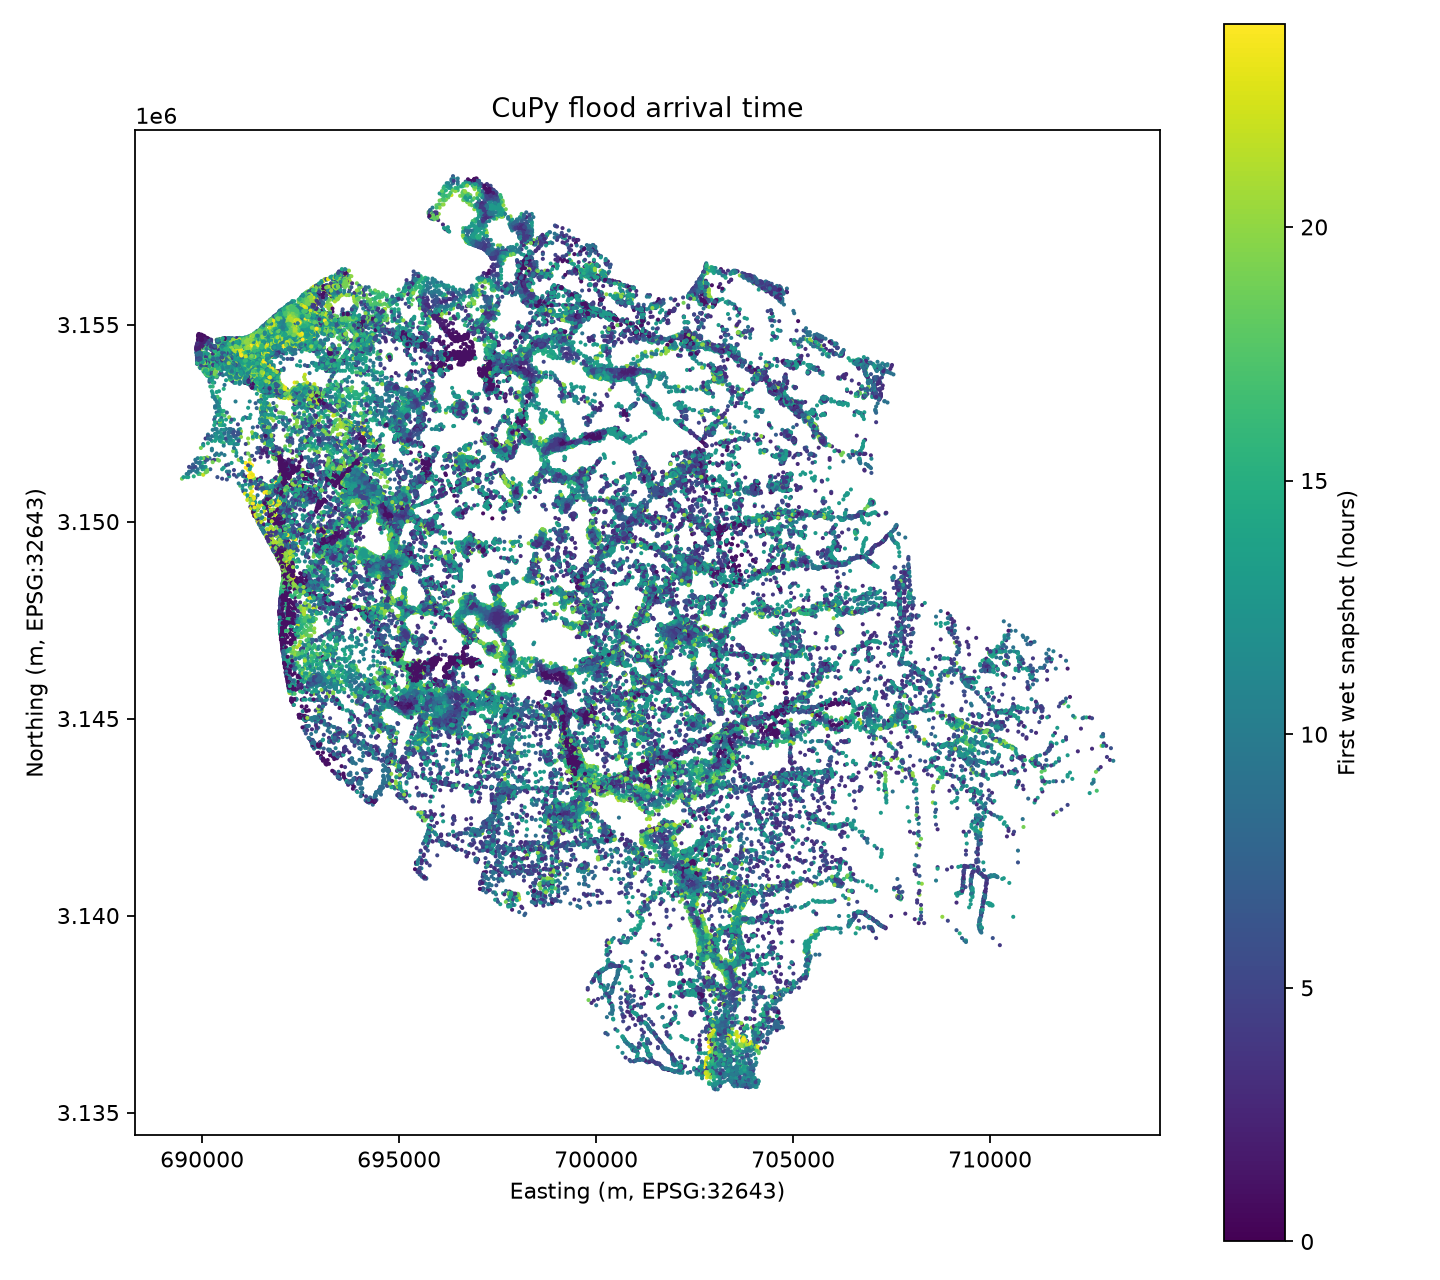
\includegraphics[width=\linewidth]{12_arrival_time.png}
\caption{Derived arrival time.}
\end{subfigure}
\caption[Thresholded flood extent and arrival-time products.]{Thresholded flood extent and
arrival-time products.}
\label{fig:extent}
\end{figure}

\section{Flood duration and velocity diagnostics}
Flood duration counts the stored hourly states in which each cell exceeds the registered
\SI{0.05}{\metre} wet threshold. Because the first stored state occurs after one second and
the remaining targets are hourly, the maximum count is 25; the product is a count of wet
snapshots, not a continuously integrated duration. Long-duration cells form connected and
localized corridors within the active domain, whereas most triangles never cross the
threshold. This pattern is consistent with the final wet count being much smaller than the
817,573 active cells.

The event maximum-speed product is calculated from the depth-averaged velocity history. In
the CuPy archive its domain-wide maximum is \SI{1.712713}{\metre\per\second}, its
all-cell mean is \SI{0.0421213}{\metre\per\second}, and all 981,880 entries are finite.
For JAX, the corresponding maximum and mean are 1.712712 and
\SI{0.0421171}{\metre\per\second}. Both maxima remain below the model's registered
\SI{5}{\metre\per\second} safety ceiling, so the reported event maximum is not equal to
the cap.

\begin{figure}[htbp]
\centering
\begin{subfigure}[t]{0.49\textwidth}
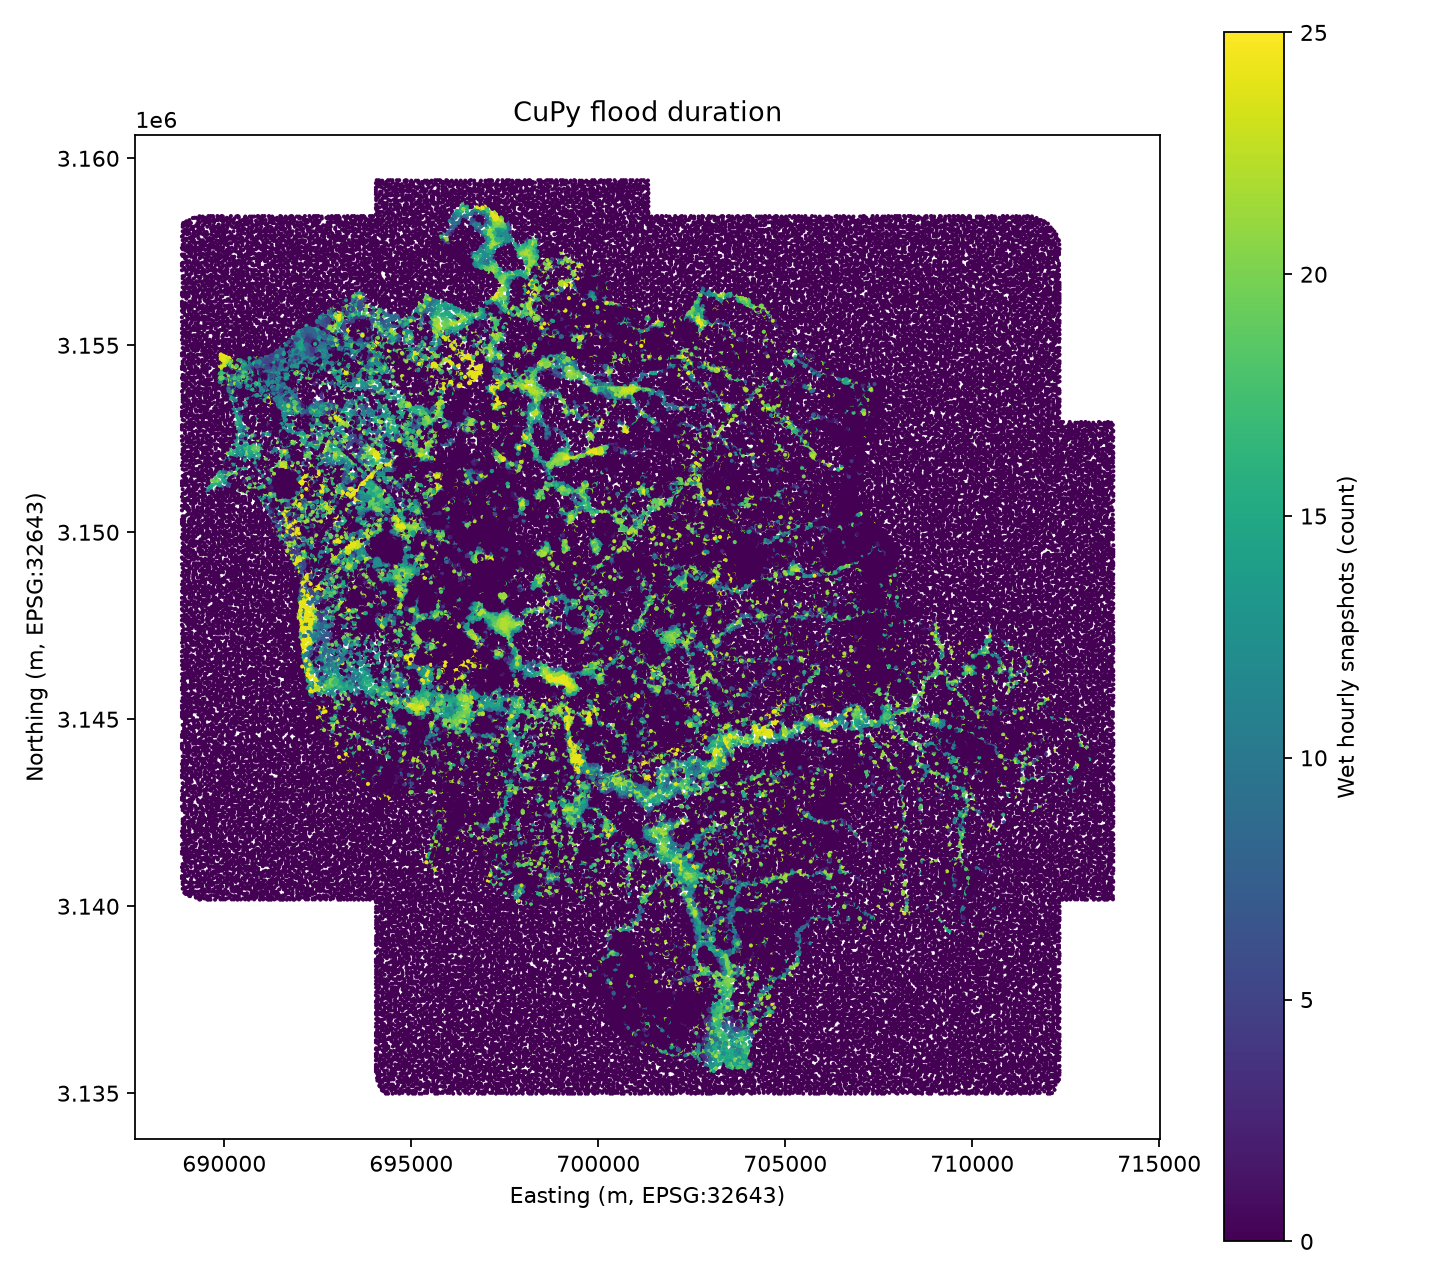
\includegraphics[width=\linewidth]{13_flood_duration.png}
\caption{Wet-snapshot count at the 0.05 m threshold.}
\end{subfigure}\hfill
\begin{subfigure}[t]{0.49\textwidth}
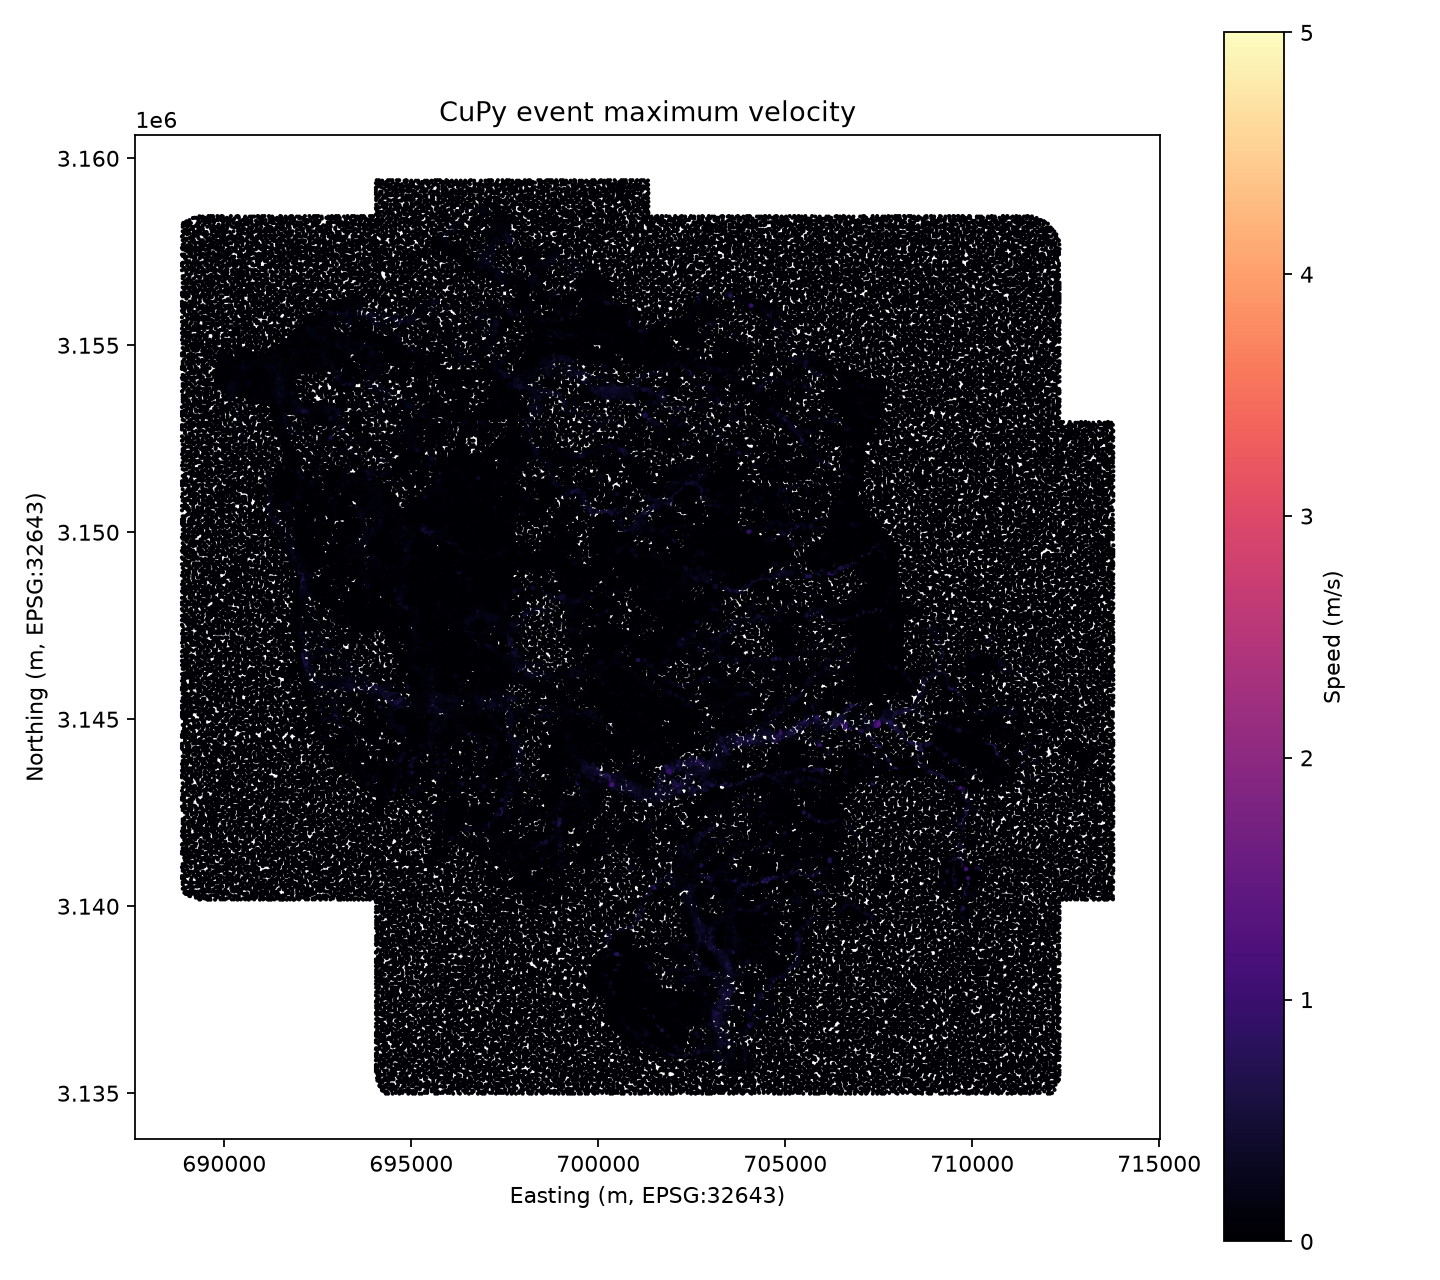
\includegraphics[width=\linewidth]{14_velocity.png}
\caption{Event maximum depth-averaged speed.}
\end{subfigure}
\caption[Duration and velocity products.]{Derived CuPy duration and maximum-velocity
products from the preserved 24-hour histories.}
\label{fig:durationvelocity}
\end{figure}

The velocity map should be interpreted as a hydraulic-model diagnostic rather than a
pedestrian or vehicle hazard classification. No external hazard standard was imposed in the
completed experiment, and velocity alone omits depth and exposure. Likewise, a wet-snapshot
count supports comparison within this output schedule but cannot resolve sub-hourly arrival
or recession between saved states.

\section{Mass-balance accounting}
The CuPy compatible ledger residual was \SI{136495.864}{\cubic\metre}, or 0.269684\% of its
registered denominator. The JAX compatible residual was \SI{147573.342}{\cubic\metre}, or
0.291569\%. JAX additionally tracks ending recharge storage explicitly; including
\SI{63394.368}{\cubic\metre} gives a complete JAX residual of
\SI{84178.974}{\cubic\metre}, or 0.166317\%. The parity gate is a regression criterion: the
candidate compatible residual ratio may exceed the CuPy ratio by no more than 0.001. It is
not an assertion that absolute residual must be below 0.1\%. The observed increase was
0.000218855 and passed.

The ledger includes rainfall, infiltration, external inflow, boundary flux, inlet capture,
surcharge, outfalls, recharge and ending surface/network storage. This explicit accounting
makes it possible to locate imbalance without treating the final surface volume as the
entire system mass.

\begin{table}[H]
\centering
\caption[Detailed 24-hour mass-ledger terms.]{Detailed cumulative mass-ledger terms. Signs
in the source reports follow their native conventions; magnitudes are shown for named
losses and exchanges.}
\label{tab:ledgerdetail}
\footnotesize
\begin{tabular}{|l|r|r|}
\hline
\textbf{Ledger term (m$^3$)} & \textbf{CuPy} & \textbf{JAX} \\
\hline\hline
Initial drainage-node storage & 2,128,865.685 & 2,128,865.750 \\ \hdashline[0.4pt/1.2pt]
Rainfall input & 47,701,360.545 & 47,701,532.000 \\ \hdashline[0.4pt/1.2pt]
External boundary inflow & 783,082.540 & 783,082.500 \\ \hdashline[0.4pt/1.2pt]
Net outward boundary transfer & 21,060,985.221 & 21,051,882.000 \\ \hdashline[0.4pt/1.2pt]
Infiltration loss & 4,545,656.989 & 4,545,672.500 \\ \hdashline[0.4pt/1.2pt]
Outfall discharge & 1,060,887.868 & 1,060,836.750 \\ \hdashline[0.4pt/1.2pt]
Overflow / surcharge diagnostic & 16,184,457.202 & 16,182,797.000 \\ \hdashline[0.4pt/1.2pt]
Final surface storage & 23,377,569.249 & 23,375,823.126 \\ \hdashline[0.4pt/1.2pt]
Final drainage-node storage & 420,425.063 & 420,421.469 \\ \hdashline[0.4pt/1.2pt]
Final recharge storage & not explicit in compatible ledger & 63,394.368 \\
\hline
\end{tabular}
\end{table}

Rainfall is the largest recorded external input, while net boundary transfer is the largest
named outward term. The overflow/surcharge values describe internal network-to-surface
exchange and must not be added as a new external source when closing the whole-system
balance. At 24 hours, surface storage is approximately \SI{23.38e6}{\cubic\metre} and node
storage approximately \SI{0.420e6}{\cubic\metre} in both implementations.

\begin{figure}[htbp]
\centering
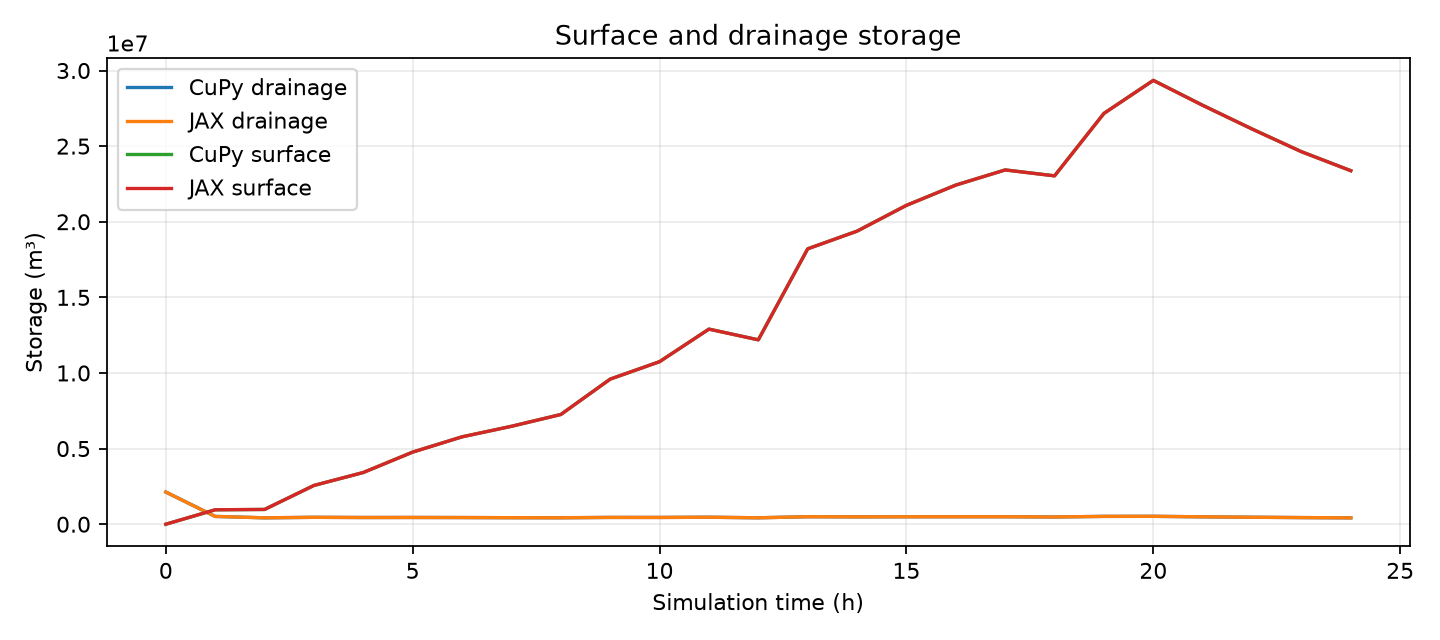
\includegraphics[width=0.88\textwidth]{15_storage.png}
\caption[Surface and drainage storage histories.]{Surface and drainage-node storage through
the production event. The nearly overlapping backend curves provide a time-resolved view of
the parity summarized by scalar gates.}
\label{fig:storage}
\end{figure}

Surface storage rises in steps that follow the temporally varying rainfall and other source
terms, reaches its largest plotted value near hour 20, and then declines toward the final
state. Drainage storage begins from the topology-defined nonzero initial condition, changes
rapidly during the first hour, and remains much smaller than surface storage on the common
vertical scale. The CuPy and JAX curves visually overlap throughout; the numerical parity
chapter quantifies the remaining differences rather than relying on visual agreement.

% =============================================================================
\chapter{Numerical Parity and Repeatability}\label{chap:parity}
% =============================================================================
\section{Cross-backend parity}
All eight registered gates passed. The largest hourly depth RMSE was only 1.96\% of the
\SI{0.05}{\metre} limit, and the minimum CSI exceeded its 0.95 limit by 0.048. The final
surface-volume difference was approximately \SI{-1746.12}{\cubic\metre}, corresponding to
-0.00747\%, while the maximum absolute hourly volume error was 0.03329\%.

\begin{table}[H]
\centering
\caption[Approved parity gates and observations.]{Approved parity gates and observed
values.}
\label{tab:gates}
\footnotesize
\begin{tabularx}{\textwidth}{|X|r|r|c|}
\hline
\textbf{Gate} & \textbf{Approved limit} & \textbf{Observed} & \textbf{Result} \\
\hline\hline
Minimum hourly flood-extent CSI & $\geq0.95$ & 0.998031 & Pass \\ \hdashline[0.4pt/1.2pt]
Maximum hourly depth RMSE & $\leq0.05$ m & 0.000979348 m & Pass \\ \hdashline[0.4pt/1.2pt]
Maximum hourly volume error & $\leq2\%$ & 0.033294\% & Pass \\ \hdashline[0.4pt/1.2pt]
Finite/non-negative depth & min $\geq-10^{-7}$ m & finite/non-negative & Pass \\ \hdashline[0.4pt/1.2pt]
Residual-ratio regression & increase $\leq0.001$ & 0.000218855 & Pass \\ \hdashline[0.4pt/1.2pt]
Maximum-depth relative error & $\leq5\%$ & 0.0000810\% & Pass \\ \hdashline[0.4pt/1.2pt]
Snapshot-time mismatch & $\leq1$ s & 0.318359 s & Pass \\ \hdashline[0.4pt/1.2pt]
Source--sink ledger difference & $\leq2\%$ & 1.543653\% & Pass \\
\hline
\end{tabularx}
\end{table}

\begin{figure}[htbp]
\centering
\begin{subfigure}[t]{0.70\textwidth}
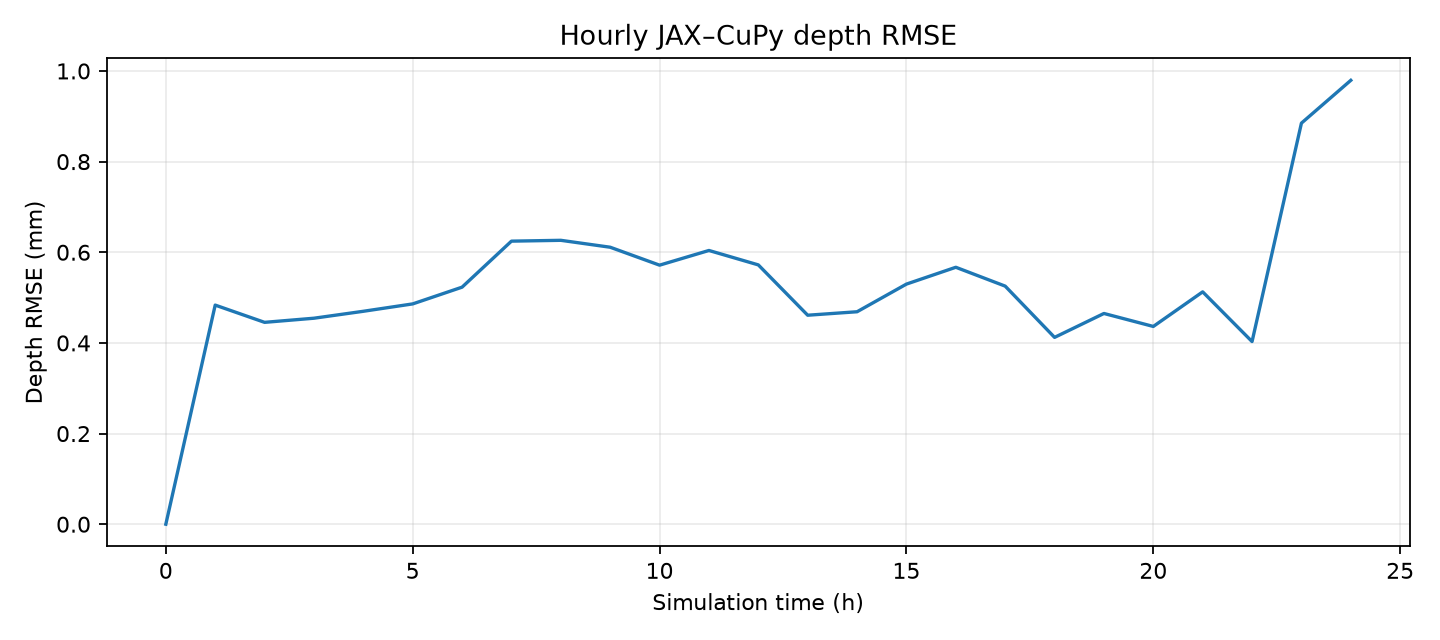
\includegraphics[width=\linewidth]{16_parity_rmse.png}
\caption{Hourly depth RMSE.}
\end{subfigure}\hfill
\begin{subfigure}[t]{0.49\textwidth}
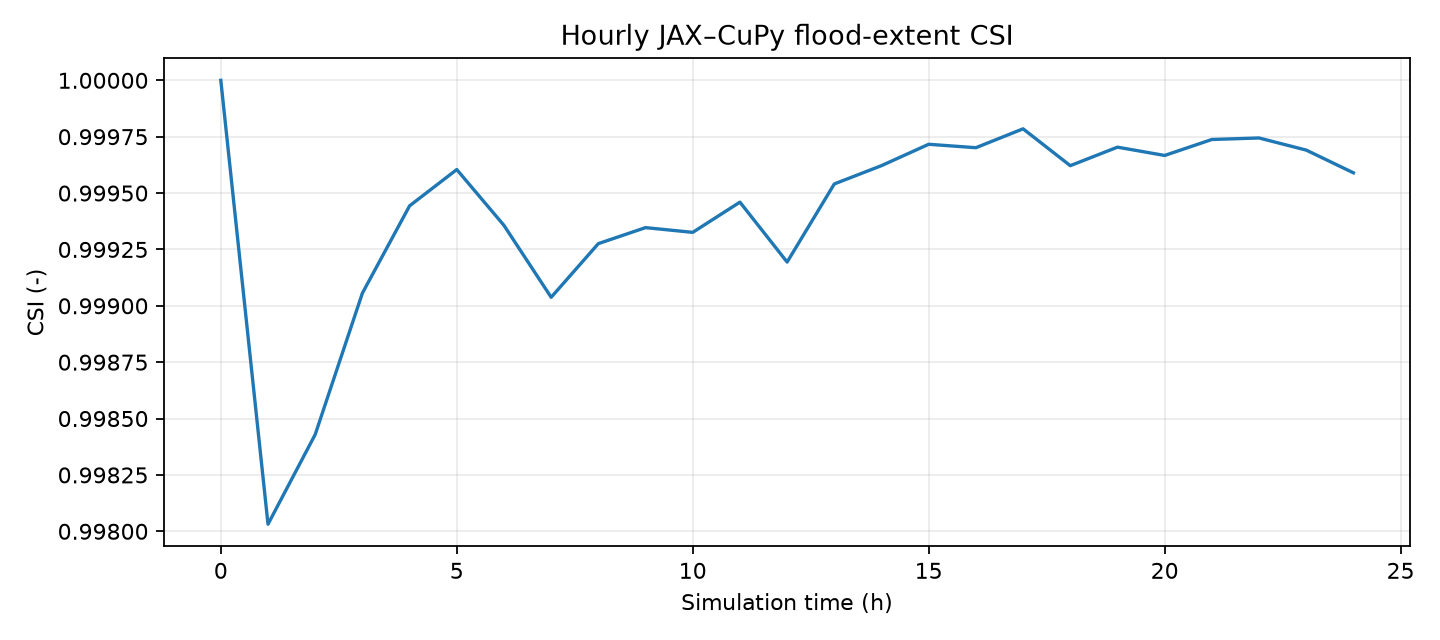
\includegraphics[width=\linewidth]{17_parity_csi.png}
\caption{Hourly flood-extent CSI.}
\end{subfigure}
\caption[Cross-backend parity through the event.]{Cross-backend parity through the
24-hour event.}
\label{fig:parity}
\end{figure}

\section{Spatial differences}
At the final state, depth RMSE was \SI{0.000979348}{\metre}, CSI was 0.999590 and the
domain-wide maximum-depth values differed by \SI{7.63e-6}{\metre}. Local differences are
spatially heterogeneous and may be amplified near wet--dry transitions even when global
errors remain small. The difference map is therefore more informative than a single scalar
alone.

\begin{figure}[H]
\centering
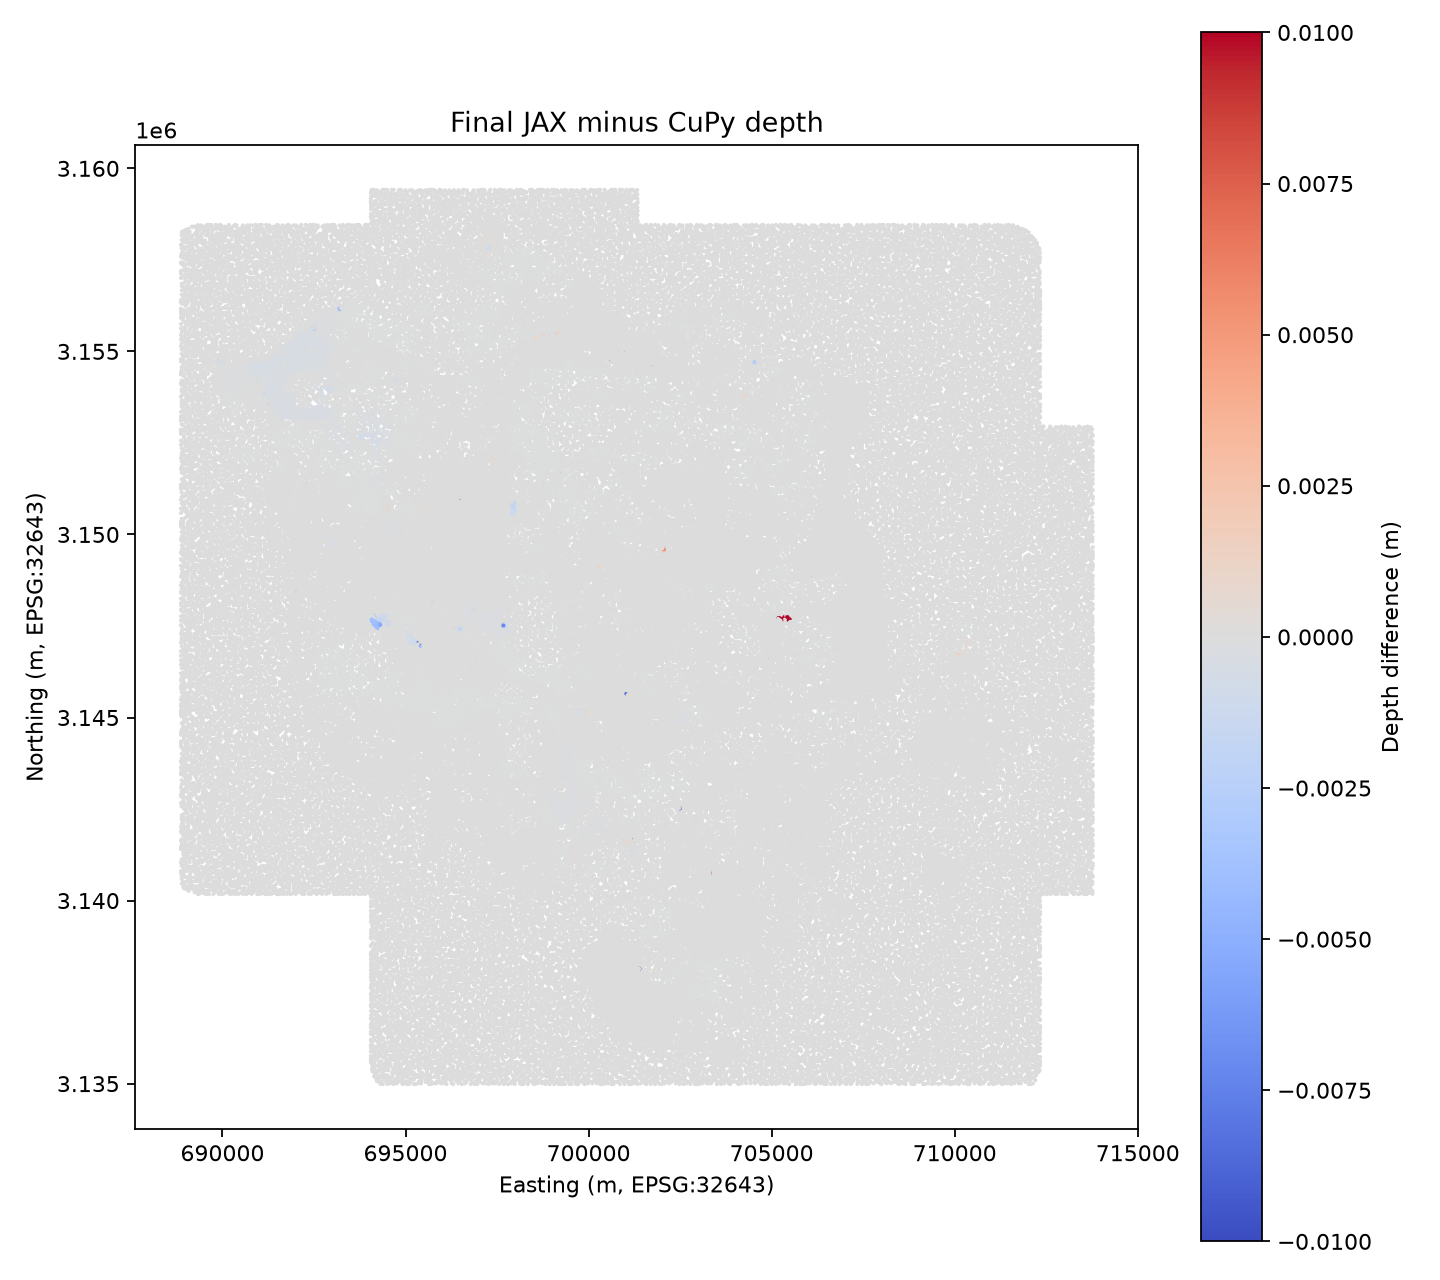
\includegraphics[width=0.58\textwidth]{18_spatial_depth_difference.png}
\caption[Spatial difference between JAX and CuPy depths.]{Spatial difference between final
JAX and CuPy depths. CuPy is the implementation reference, not an observed truth field.}
\label{fig:diff}
\end{figure}

\section{Within-backend repeatability}
Independent run-B executions passed the pre-existing repeatability criteria for both
backends. CuPy produced RMSE \SI{0.000416766}{\metre}, minimum CSI 0.998740 and maximum
snapshot offset \SI{0.354492}{\second}; its timestep count differed by 28. JAX produced RMSE
\SI{0.000406100}{\metre}, minimum CSI 0.998031 and maximum snapshot offset
\SI{0.337891}{\second}; its timestep count differed by 24.

\begin{table}[H]
\centering
\caption[Within-backend repeatability.]{Independent 24-hour within-backend repeatability.}
\label{tab:repeat}
\small
\begin{tabular}{|l|r|r|r|c|c|}
\hline
\textbf{Backend} & \textbf{RMSE (m)} & \textbf{Minimum CSI} & \textbf{Offset (s)} &
\textbf{$\Delta$ steps} & \textbf{Bitwise} \\
\hline\hline
CuPy & 0.000416766 & 0.998740 & 0.354492 & 28 & No \\ \hdashline[0.4pt/1.2pt]
JAX  & 0.000406100 & 0.998031 & 0.337891 & 24 & No \\
\hline
\end{tabular}
\end{table}

Neither output archive was byte-identical. The evidence shows association with adaptive
timestep and snapshot-time divergence, but it does not isolate a lower-level cause among
GPU reduction order, floating-point non-associativity and wet--dry sensitivity. The correct
classification is therefore \emph{numerically repeatable within the approved criteria, but
not bitwise deterministic}.

\section{Interpretation of localized differences}
Global norms and spatial extremes answer different questions. The repeat-run maximum
absolute depth differences reached \SI{0.283989}{\metre} for CuPy and
\SI{0.603012}{\metre} for JAX, even though their domain-wide RMSE values remained below
\SI{0.000417}{\metre}. This combination indicates that the largest changes are localized
rather than representative of the entire mesh. Reporting only RMSE would conceal those
outliers; reporting only the maximum would incorrectly imply a domain-wide discrepancy.
The simultaneous CSI values above 0.998 show that thresholded inundation support remained
very similar.

Wet--dry transitions are a plausible location for amplified local differences because a
small depth change can alter whether momentum is retained, whether an inlet has water
available, and which adaptive timestep is selected. 

\newpage

The two repeats also had different step
counts and slightly different snapshot times. These observations establish association, not
a proven low-level cause. Isolating the cause would require controlled kernel-level tests of
reduction order, timestep selection and threshold crossings, which were not part of the
completed experiment.

The parity conclusion therefore rests on multiple complementary metrics: RMSE and MAE for
distributed depth error, CSI for flood support, volume and ledger terms for conservation,
maximum-depth comparison for the event extreme, and time alignment for snapshot validity.
Agreement across these metrics justifies numerical equivalence within the approved gates,
while the lack of byte identity is retained as a separate and transparent result.

\begin{table}[H]
\centering
\caption[Selected hourly parity observations.]{Selected time-resolved observations from the
complete 25-state parity table.}
\label{tab:selectedhourly}
\footnotesize
\begin{tabular}{|r|r|r|r|r|}
\hline
\textbf{Time (h)} & \textbf{Depth MAE (m)} & \textbf{Depth RMSE (m)} &
\textbf{Flood CSI} & \textbf{$\Delta V_s$ (m$^3$)} \\
\hline\hline
0$^*$ & $4.6920\times10^{-10}$ & $3.9743\times10^{-8}$ & 1.000000 & $-0.0046$ \\
\hdashline[0.4pt/1.2pt]
1 & $8.8698\times10^{-6}$ & $4.8343\times10^{-4}$ & 0.998031 & 104.395 \\
\hdashline[0.4pt/1.2pt]
6 & $1.5106\times10^{-5}$ & $5.2301\times10^{-4}$ & 0.999357 & $-940.855$ \\
\hdashline[0.4pt/1.2pt]
12 & $2.7740\times10^{-5}$ & $5.7215\times10^{-4}$ & 0.999194 & $-3545.801$ \\
\hdashline[0.4pt/1.2pt]
18 & $3.1494\times10^{-5}$ & $4.1220\times10^{-4}$ & 0.999622 & $-4509.684$ \\
\hdashline[0.4pt/1.2pt]
24 & $5.2020\times10^{-5}$ & $9.7935\times10^{-4}$ & 0.999590 & $-1746.123$ \\
\hline
\end{tabular}

\vspace{1mm}
\parbox{0.94\textwidth}{\footnotesize $^*$The first stored state is at 1 s and is labelled
as the initial output in the package. $\Delta V_s=V_{s,JAX}-V_{s,CuPy}$.}
\end{table}

The selected rows illustrate why acceptance was evaluated over the entire event. The minimum
CSI occurred near the beginning rather than at the final output, whereas the largest depth
RMSE occurred at 24 hours. Surface-volume difference also changed sign and magnitude through
time. A final-state-only comparison would therefore miss the worst extent agreement and
would provide no evidence that the intermediate trajectories remained close.

\begin{table}[H]
\centering
\caption[Complementary meaning of parity metrics.]{Why no single metric is sufficient for
the completed numerical-equivalence decision.}
\label{tab:metricroles}
\footnotesize
\begin{tabularx}{\textwidth}{|p{0.23\textwidth}|p{0.31\textwidth}|X|}
\hline
\textbf{Metric family} & \textbf{Question answered} & \textbf{Failure it can reveal} \\
\hline\hline
MAE, RMSE and relative $L_2$ & How different are distributed depth fields? & Broad bias or
accumulated field disagreement \\ \hdashline[0.4pt/1.2pt]
CSI, precision and recall & Do the backends inundate the same cells? & Shifted wet--dry
fronts hidden by a small domain-average error \\ \hdashline[0.4pt/1.2pt]
Surface volume and ledger & Are integrated water quantities consistent? & Source, sink or
exchange accounting mismatch \\ \hdashline[0.4pt/1.2pt]
Maximum depth & Is the event extreme reproduced? & Local peak amplification or suppression
\\ \hdashline[0.4pt/1.2pt]
Snapshot-time offset & Are fields compared at equivalent times? & Apparent spatial error
caused by adaptive-clock misalignment \\
\hline
\end{tabularx}
\end{table}

% =============================================================================
\chapter{GPU Performance Comparison}\label{chap:performance}
% =============================================================================
\section{Completed secondary benchmark}
The complete repeated comparison used a 60-minute production workload, three warm-ups and
ten accepted measurements for each backend. All twenty measured results passed correctness
checks. CuPy median solver runtime was \SI{17.267041}{\second}; JAX median runtime was
\SI{18.212524}{\second}. With
\begin{equation}
 \Delta_{J/C}=100\left(\frac{T_J}{T_C}-1\right),
\end{equation}
the measured difference is 5.475648\%, meaning JAX was slower for this specific workload,
device and software environment.

\begin{table}[H]
\centering
\caption[Secondary repeated GPU benchmark.]{Secondary 60-minute production benchmark.}
\label{tab:benchmark}
\renewcommand{\arraystretch}{0.95}
\small
\begin{tabular}{|l|r|r|}
\hline
\textbf{Statistic} & \textbf{CuPy} & \textbf{JAX} \\
\hline\hline
Warm-ups / measurements & 3 / 10 & 3 / 10 \\ \hdashline[0.4pt/1.2pt]
Mean runtime (s) & 17.333616 & 18.215309 \\ \hdashline[0.4pt/1.2pt]
Median runtime (s) & 17.267041 & 18.212524 \\ \hdashline[0.4pt/1.2pt]
Minimum--maximum (s) & 16.983008--17.854433 & 18.185589--18.251359 \\ \hdashline[0.4pt/1.2pt]
Population standard deviation (s) & 0.333464 & 0.021280 \\ \hdashline[0.4pt/1.2pt]
Interquartile range (s) & 0.628316 & 0.025221 \\ \hdashline[0.4pt/1.2pt]
Coefficient of variation & 0.019238 & 0.001168 \\ \hdashline[0.4pt/1.2pt]
Median steps per second & 758.443 & 718.515 \\ \hdashline[0.4pt/1.2pt]
Simulated h per wall-clock h & 208.507 & 197.666 \\
\hline
\end{tabular}
\end{table}

\begin{figure}[H]
\centering
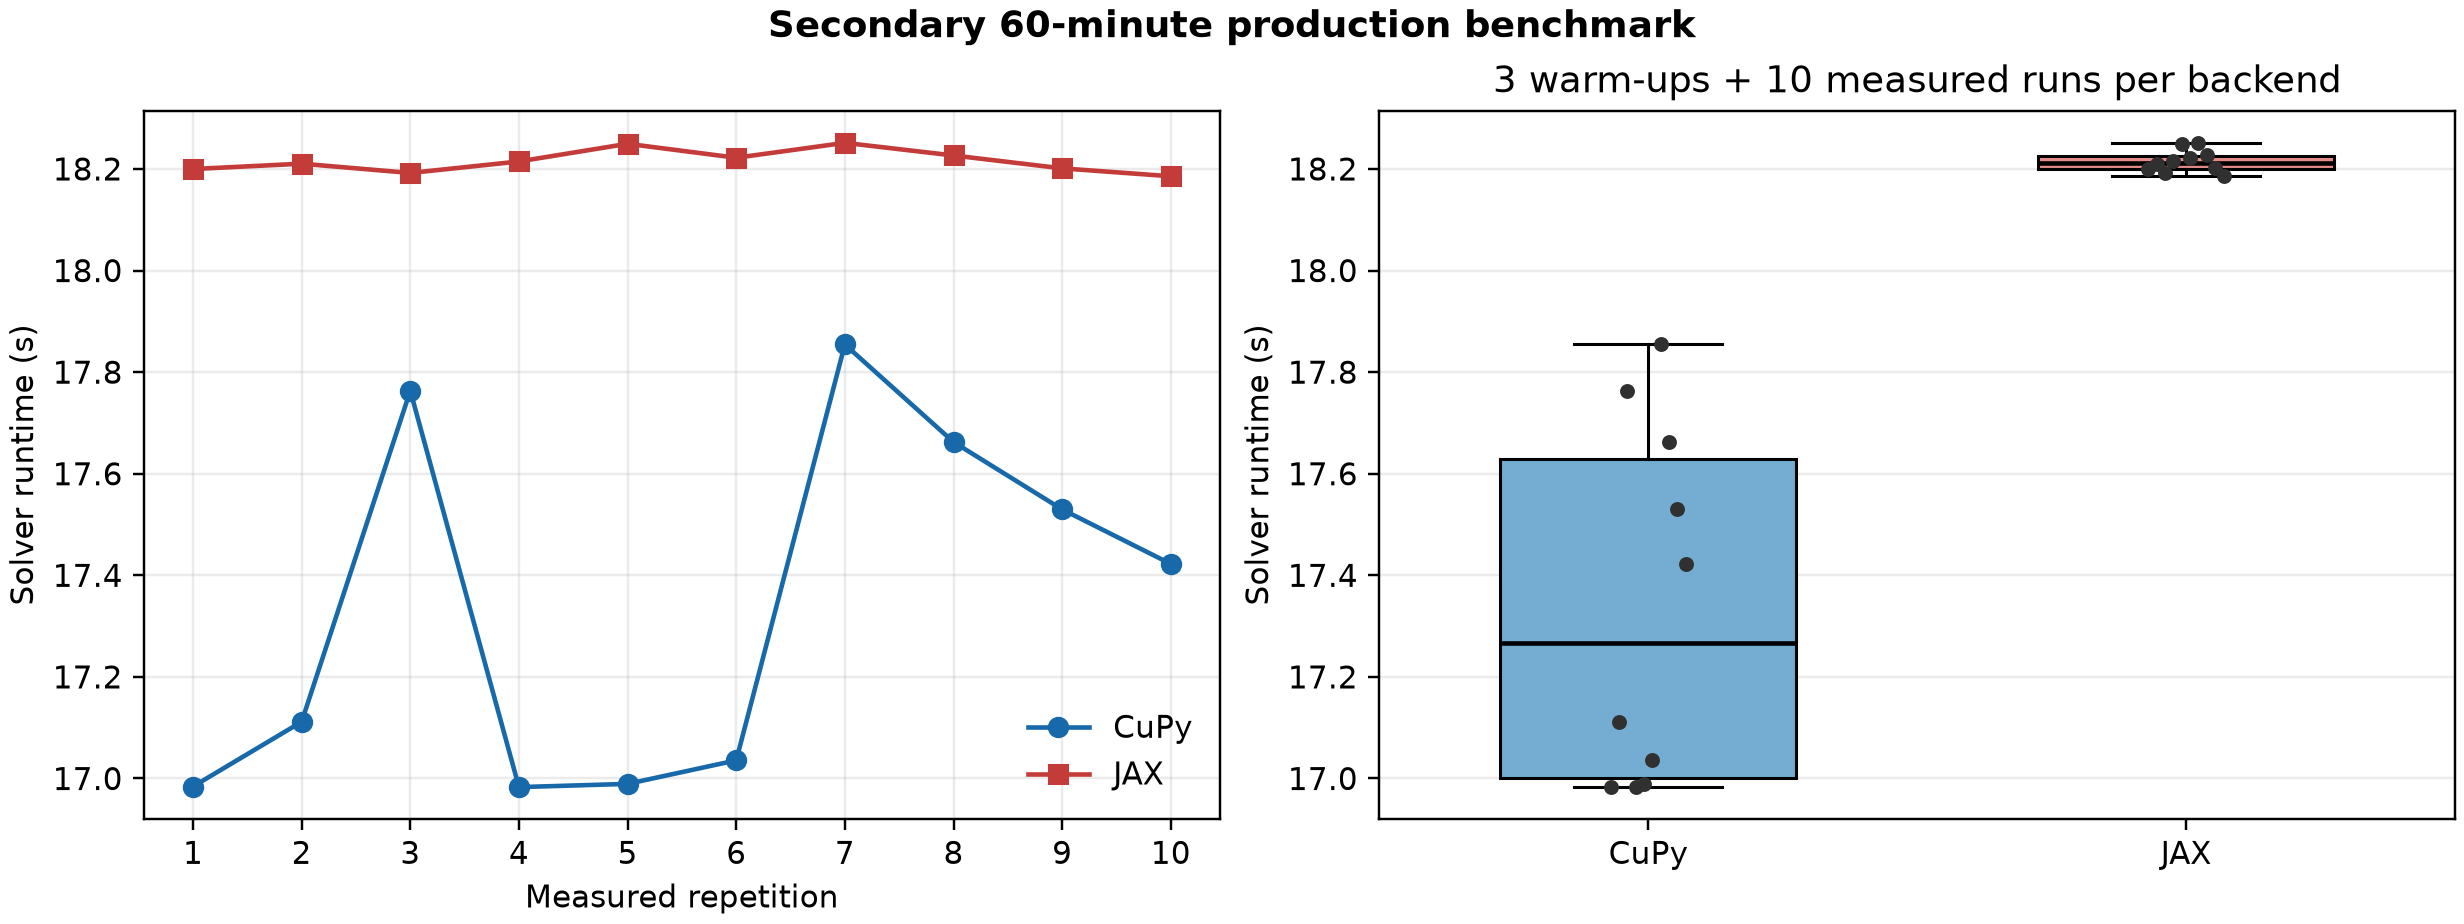
\includegraphics[width=0.88\textwidth]{19_runtime_distribution.png}
\caption[Runtime distribution for the secondary benchmark.]{Measured solver runtimes for
ten repetitions per backend after three warm-ups. The figure was generated from the verified
\texttt{benchmarks/secondary\_60min/benchmark\_results.csv} records.}
\label{fig:runtime}
\end{figure}

\section{Interpretation}
The result does not imply that CuPy is universally faster than JAX. CuPy benefits here from
production-specific fused CUDA kernels, while JAX provides compiler-managed fusion,
functional transformations and a path toward differentiable or ML-coupled workflows. The
CuPy timings show greater run-to-run dispersion, whereas the JAX timings are tightly
clustered, but ten measurements are insufficient for broad hardware-general conclusions.
The benchmark supports only the claim that CuPy had the lower median solver runtime in the
completed secondary experiment.

\newpage

\section{Unfinished official 24-hour benchmark}
\enlargethispage{4\baselineskip}
The official protocol required three warm-ups and ten 24-hour measurements per backend.
CuPy completed ten measurements (median \SI{426.089}{\second}); JAX completed only three
(partial median \SI{448.328}{\second}) before the stop. The JAX sample is incomplete, so no
official 24-hour ratio, confidence interval or significance test is reported. The single
timings in \cref{tab:production} also remain descriptive rather than benchmark results. These
partial counts and timings are retained in the supplementary interrupted-run progress record,
separate from the completed secondary-benchmark evidence.

% =============================================================================
\chapter{ANUGA Numerical Reference}\label{chap:anuga}
% =============================================================================
ANUGA is an external finite-volume shallow-water model and is neither the CuPy nor JAX
implementation \cite{anuga,zoppou1999}. Version 3.3.10 was run independently on compatible
two-triangle controlled cases. Still-water and rainfall-only comparisons passed the existing
absolute mass criterion of \SI{5e-8}{\cubic\metre}. The moving-water dam-break comparison is
descriptive because reconstruction and numerical flux choices differ.

\begin{table}[H]
\centering
\caption[Controlled-case ANUGA--JAX evidence.]{Available controlled-case ANUGA--JAX
evidence. \anugasource}
\label{tab:anuga}
\footnotesize
\begin{tabularx}{\textwidth}{|X|r|r|X|}
\hline
\textbf{Case} & \textbf{Depth RMSE (m)} & \textbf{Volume difference (m$^3$)} &
\textbf{Classification} \\
\hline\hline
Still water & $2.980232\times10^{-9}$ & $2.980232\times10^{-9}$ & Criterion passed \\ \hdashline[0.4pt/1.2pt]
Rainfall only & $5.518733\times10^{-12}$ & $5.518733\times10^{-12}$ & Criterion passed \\ \hdashline[0.4pt/1.2pt]
Moving-water dam break & $6.398733\times10^{-3}$ & $-3.725290\times10^{-9}$ & Descriptive only \\ \hdashline[0.4pt/1.2pt]
Terrain lake at rest & --- & --- & ANUGA-only diagnostic; zero stage drift \\
\hline
\end{tabularx}
\end{table}

A full production-domain cross-model run was deliberately not executed. The current ANUGA
adapter cannot identically represent the production drainage, recharge, surcharge, outfall,
external-hydrograph and outflow-only boundary system. Removing those components would form
a different model and would not be a valid production comparison. The available ANUGA work
supports limited implementation verification on compatible physics; it is not validation
against real flood observations.

% =============================================================================
\chapter{Limitations and Future Work}\label{chap:limits}
% =============================================================================
The strongest limitation is the absence of compatible observations. Without surveyed water
levels, flood outlines, discharge hydrographs or arrival times, the model cannot be assigned
physical predictive accuracy. The DEM vertical datum is undocumented, which limits absolute
water-level interpretation. Only one production rainfall event is available, so the results
do not quantify event-to-event generalization and cannot support leakage-controlled
production AI splits.

The official repeated 24-hour benchmark is incomplete for JAX. The complete 60-minute
benchmark is valid but secondary and hardware-specific. Numerical repeatability was achieved
without byte-level identity, and the low-level origin of the small divergence was not
isolated. The ANUGA reference is restricted to small compatible cases rather than the full
production drainage model.

Future work should prioritize observed flood data with documented spatial and temporal
support, DEM vertical-datum confirmation, and independent rainfall events. Calibration and
validation must use separate events. The remaining seven JAX measurements should then be
completed before publishing an official 24-hour timing comparison. Multiple GPUs and
software versions would establish performance portability. If enough independent events
become available, complete-event train/validation/test partitions can support mesh-aware AI
forecasting without temporal leakage. Any surrogate should be evaluated against persistence
and physics-only baselines and should preserve uncertainty and failure reporting.

% =============================================================================
\chapter{Conclusions}\label{chap:conclusion}
% =============================================================================
This project implemented the same production urban flood model through CuPy/CUDA and
JAX/XLA on a single GPU. The executed model includes the complete triangular surface,
terrain, spatial roughness, rainfall, Horton infiltration, recharge, dynamic drainage,
surcharge, outfalls, external inflow and boundary treatment.

The central numerical objective was achieved: all eight cross-backend parity gates passed.
The final depth RMSE was \SI{0.000979348}{\metre}, final flood-extent CSI was 0.999590 and
the domain-wide maximum depths agreed to approximately \SI{7.63e-6}{\metre}. Both backends
also passed independent 24-hour numerical repeatability criteria, although neither was
bitwise deterministic. The software baseline passed 111 tests, with 37 explicitly classified
skips and no failures or errors.

The complete secondary repeated benchmark showed CuPy median runtime
\SI{17.267}{\second} and JAX median runtime \SI{18.213}{\second}; JAX was 5.476\% slower on
the tested 60-minute workload. This is the defensible performance result. The incomplete
24-hour repeated benchmark is reported only as unfinished evidence. Controlled ANUGA cases
provide limited independent numerical support but not production physical validation.

Accordingly, the project is complete as a GPU numerical implementation, verification,
repeatability and secondary performance study. It is not complete as an observationally
validated forecasting system or production AI study. This qualified conclusion is more
scientifically precise than treating successful computation as proof of real-world accuracy.

% =============================================================================
\chapter*{Reproducibility and Evidence Statement}
\addcontentsline{toc}{chapter}{Reproducibility and Evidence Statement}
The authoritative source for the completed production runs, parity, repeatability, software
verification and secondary benchmark is the repository folder
\path{HF_CUPY_JAX_COMPLETED_PROJECT}. The project repository is publicly available at
\url{https://github.com/arsanjeevk/gpu-urban-flood-cupy-jax} \cite{projectrepo}.
Key evidence consists of \texttt{COMPLETION\_ADDENDUM.md}, test output and summary,
backend run reports, hourly parity tables, validation gates, mass ledgers, repeatability
metrics, raw secondary benchmark measurements, environment metadata, source manifests and
checksums. Supplementary ANUGA controlled-case evidence is retained in
\texttt{Ravi-20260903T125449Z-1-001/Ravi/evidence}; the interrupted official 24-hour benchmark
counts and partial timings are retained in that package's \texttt{CURRENT\_PROGRESS\_REPORT.md}.
Neither supplementary record overrides the completed-project results.

The packaged archive SHA-256 checksum is
\begin{center}\small
\path{d9b4656055b728de582be8d5fb53892cff659d7ef5a5f29312365bb15bb7476c}.
\end{center}

\begin{table}[H]
\centering
\caption[Evidence retained with the completed project.]{Evidence groups used to construct
and independently check the report.}
\label{tab:evidencefiles}
\footnotesize
\begin{tabularx}{\textwidth}{|p{0.25\textwidth}|X|}
\hline
\textbf{Evidence group} & \textbf{Preserved material} \\
\hline\hline
Inputs and provenance & Production configurations, rainfall series, source manifest and
asset hashes \\ \hdashline[0.4pt/1.2pt]
Simulation state & CuPy and JAX NPZ archives, run reports and array catalogue \\
\hdashline[0.4pt/1.2pt]
Numerical verification & Hourly parity table, eight validation gates, spatial-difference
arrays, mass ledgers and repeatability metrics \\ \hdashline[0.4pt/1.2pt]
Performance & Raw secondary measurements, summary statistics and benchmark protocol \\
\hdashline[0.4pt/1.2pt]
Reproduction & Software/GPU environment, test output, commands, scripts and semantic package
audit \\
\hline
\end{tabularx}
\end{table}
The report PDF is a synthesis of existing evidence: no solver or simulation output was
modified or regenerated during report preparation.

% =============================================================================
\begin{thebibliography}{99}
\addcontentsline{toc}{chapter}{References}

\bibitem{projectrepo}
S. Kumawat, \emph{GPU-Accelerated Physics-Based Urban Flood Modelling Using
CuPy/CUDA and JAX/XLA}, project source code, configurations, verification evidence and
report sources, 2026. Available:
\url{https://github.com/arsanjeevk/gpu-urban-flood-cupy-jax}.

\bibitem{leveque2002}
R. J. LeVeque, \emph{Finite Volume Methods for Hyperbolic Problems}.
Cambridge University Press, 2002. doi:10.1017/CBO9780511791253.

\bibitem{harten1983}
A. Harten, P. D. Lax, and B. van Leer, ``On upstream differencing and
Godunov-type schemes for hyperbolic conservation laws,'' \emph{SIAM Review},
vol. 25, no. 1, pp. 35--61, 1983. doi:10.1137/1025002.

\bibitem{audusse2004}
E. Audusse, F. Bouchut, M.-O. Bristeau, R. Klein, and B. Perthame,
``A fast and stable well-balanced scheme with hydrostatic reconstruction for
shallow water flows,'' \emph{SIAM Journal on Scientific Computing}, vol. 25,
no. 6, pp. 2050--2065, 2004. doi:10.1137/S1064827503431090.

\bibitem{horton1933}
R. E. Horton, ``The role of infiltration in the hydrologic cycle,''
\emph{Transactions, American Geophysical Union}, vol. 14, no. 1,
pp. 446--460, 1933. doi:10.1029/TR014i001p00446.

\bibitem{chow1959}
V. T. Chow, \emph{Open-Channel Hydraulics}. New York, NY, USA:
McGraw-Hill, 1959.

\bibitem{cupy}
R. Okuta, Y. Unno, D. Nishino, S. Hido, and C. Loomis, ``CuPy: A
NumPy-compatible library for NVIDIA GPU calculations,'' in \emph{Workshop on
Machine Learning Systems, NeurIPS}, 2017.

\bibitem{jax}
R. Frostig, M. J. Johnson, and C. Leary, ``Compiling machine learning
programs via high-level tracing,'' in \emph{Systems for Machine Learning}, 2018.

\bibitem{pytorch}
A. Paszke et al., ``PyTorch: An imperative style, high-performance deep
learning library,'' in \emph{Advances in Neural Information Processing
Systems}, vol. 32, pp. 8024--8035, 2019.

\bibitem{anuga}
S. Roberts, G. Davies, O. Nielsen, et al., \emph{ANUGA Hydrodynamic
Inundation Modelling}. Australian National University and Geoscience
Australia. Available: \url{https://github.com/anuga-community/anuga_core}.

\bibitem{zoppou1999}
C. Zoppou and S. Roberts, ``Catastrophic collapse of water supply reservoirs
in urban areas,'' \emph{Journal of Hydraulic Engineering}, vol. 125, no. 7,
pp. 686--695, 1999. doi:10.1061/(ASCE)0733-9429(1999)125:7(686).

\end{thebibliography}

\end{document}
